\documentclass[1p]{elsarticle_modified}
%\bibliographystyle{elsarticle-num}

%\usepackage[colorlinks]{hyperref}
%\usepackage{abbrmath_seonhwa} %\Abb, \Ascr, \Acal ,\Abf, \Afrak
\usepackage{amsfonts}
\usepackage{amssymb}
\usepackage{amsmath}
\usepackage{amsthm}
\usepackage{scalefnt}
\usepackage{amsbsy}
\usepackage{kotex}
\usepackage{caption}
\usepackage{subfig}
\usepackage{color}
\usepackage{graphicx}
\usepackage{xcolor} %% white, black, red, green, blue, cyan, magenta, yellow
\usepackage{float}
\usepackage{setspace}
\usepackage{hyperref}

\usepackage{tikz}
\usetikzlibrary{arrows}

\usepackage{multirow}
\usepackage{array} % fixed length table
\usepackage{hhline}

%%%%%%%%%%%%%%%%%%%%%
\makeatletter
\renewcommand*\env@matrix[1][\arraystretch]{%
	\edef\arraystretch{#1}%
	\hskip -\arraycolsep
	\let\@ifnextchar\new@ifnextchar
	\array{*\c@MaxMatrixCols c}}
\makeatother %https://tex.stackexchange.com/questions/14071/how-can-i-increase-the-line-spacing-in-a-matrix
%%%%%%%%%%%%%%%

\usepackage[normalem]{ulem}

\newcommand{\msout}[1]{\ifmmode\text{\sout{\ensuremath{#1}}}\else\sout{#1}\fi}
%SOURCE: \msout is \stkout macro in https://tex.stackexchange.com/questions/20609/strikeout-in-math-mode

\newcommand{\cancel}[1]{
	\ifmmode
	{\color{red}\msout{#1}}
	\else
	{\color{red}\sout{#1}}
	\fi
}

\newcommand{\add}[1]{
	{\color{blue}\uwave{#1}}
}

\newcommand{\replace}[2]{
	\ifmmode
	{\color{red}\msout{#1}}{\color{blue}\uwave{#2}}
	\else
	{\color{red}\sout{#1}}{\color{blue}\uwave{#2}}
	\fi
}

\newcommand{\Sol}{\mathcal{S}} %segment
\newcommand{\D}{D} %diagram
\newcommand{\A}{\mathcal{A}} %arc


%%%%%%%%%%%%%%%%%%%%%%%%%%%%%5 test

\def\sl{\operatorname{\textup{SL}}(2,\Cbb)}
\def\psl{\operatorname{\textup{PSL}}(2,\Cbb)}
\def\quan{\mkern 1mu \triangleright \mkern 1mu}

\theoremstyle{definition}
\newtheorem{thm}{Theorem}[section]
\newtheorem{prop}[thm]{Proposition}
\newtheorem{lem}[thm]{Lemma}
\newtheorem{ques}[thm]{Question}
\newtheorem{cor}[thm]{Corollary}
\newtheorem{defn}[thm]{Definition}
\newtheorem{exam}[thm]{Example}
\newtheorem{rmk}[thm]{Remark}
\newtheorem{alg}[thm]{Algorithm}

\newcommand{\I}{\sqrt{-1}}
\begin{document}

%\begin{frontmatter}
%
%\title{Boundary parabolic representations of knots up to 8 crossings}
%
%%% Group authors per affiliation:
%\author{Yunhi Cho} 
%\address{Department of Mathematics, University of Seoul, Seoul, Korea}
%\ead{yhcho@uos.ac.kr}
%
%
%\author{Seonhwa Kim} %\fnref{s_kim}}
%\address{Center for Geometry and Physics, Institute for Basic Science, Pohang, 37673, Korea}
%\ead{ryeona17@ibs.re.kr}
%
%\author{Hyuk Kim}
%\address{Department of Mathematical Sciences, Seoul National University, Seoul 08826, Korea}
%\ead{hyukkim@snu.ac.kr}
%
%\author{Seokbeom Yoon}
%\address{Department of Mathematical Sciences, Seoul National University, Seoul, 08826,  Korea}
%\ead{sbyoon15@snu.ac.kr}
%
%\begin{abstract}
%We find all boundary parabolic representation of knots up to 8 crossings.
%
%\end{abstract}
%\begin{keyword}
%    \MSC[2010] 57M25 
%\end{keyword}
%
%\end{frontmatter}

%\linenumbers
%\tableofcontents
%
\newcommand\colored[1]{\textcolor{white}{\rule[-0.35ex]{0.8em}{1.4ex}}\kern-0.8em\color{red} #1}%
%\newcommand\colored[1]{\textcolor{white}{ #1}\kern-2.17ex	\textcolor{white}{ #1}\kern-1.81ex	\textcolor{white}{ #1}\kern-2.15ex\color{red}#1	}

{\Large $\underline{11a_{196}~(K11a_{196})}$}

\setlength{\tabcolsep}{10pt}
\renewcommand{\arraystretch}{1.6}
\vspace{1cm}\begin{tabular}{m{100pt}>{\centering\arraybackslash}m{274pt}}
\multirow{5}{120pt}{
	\centering
	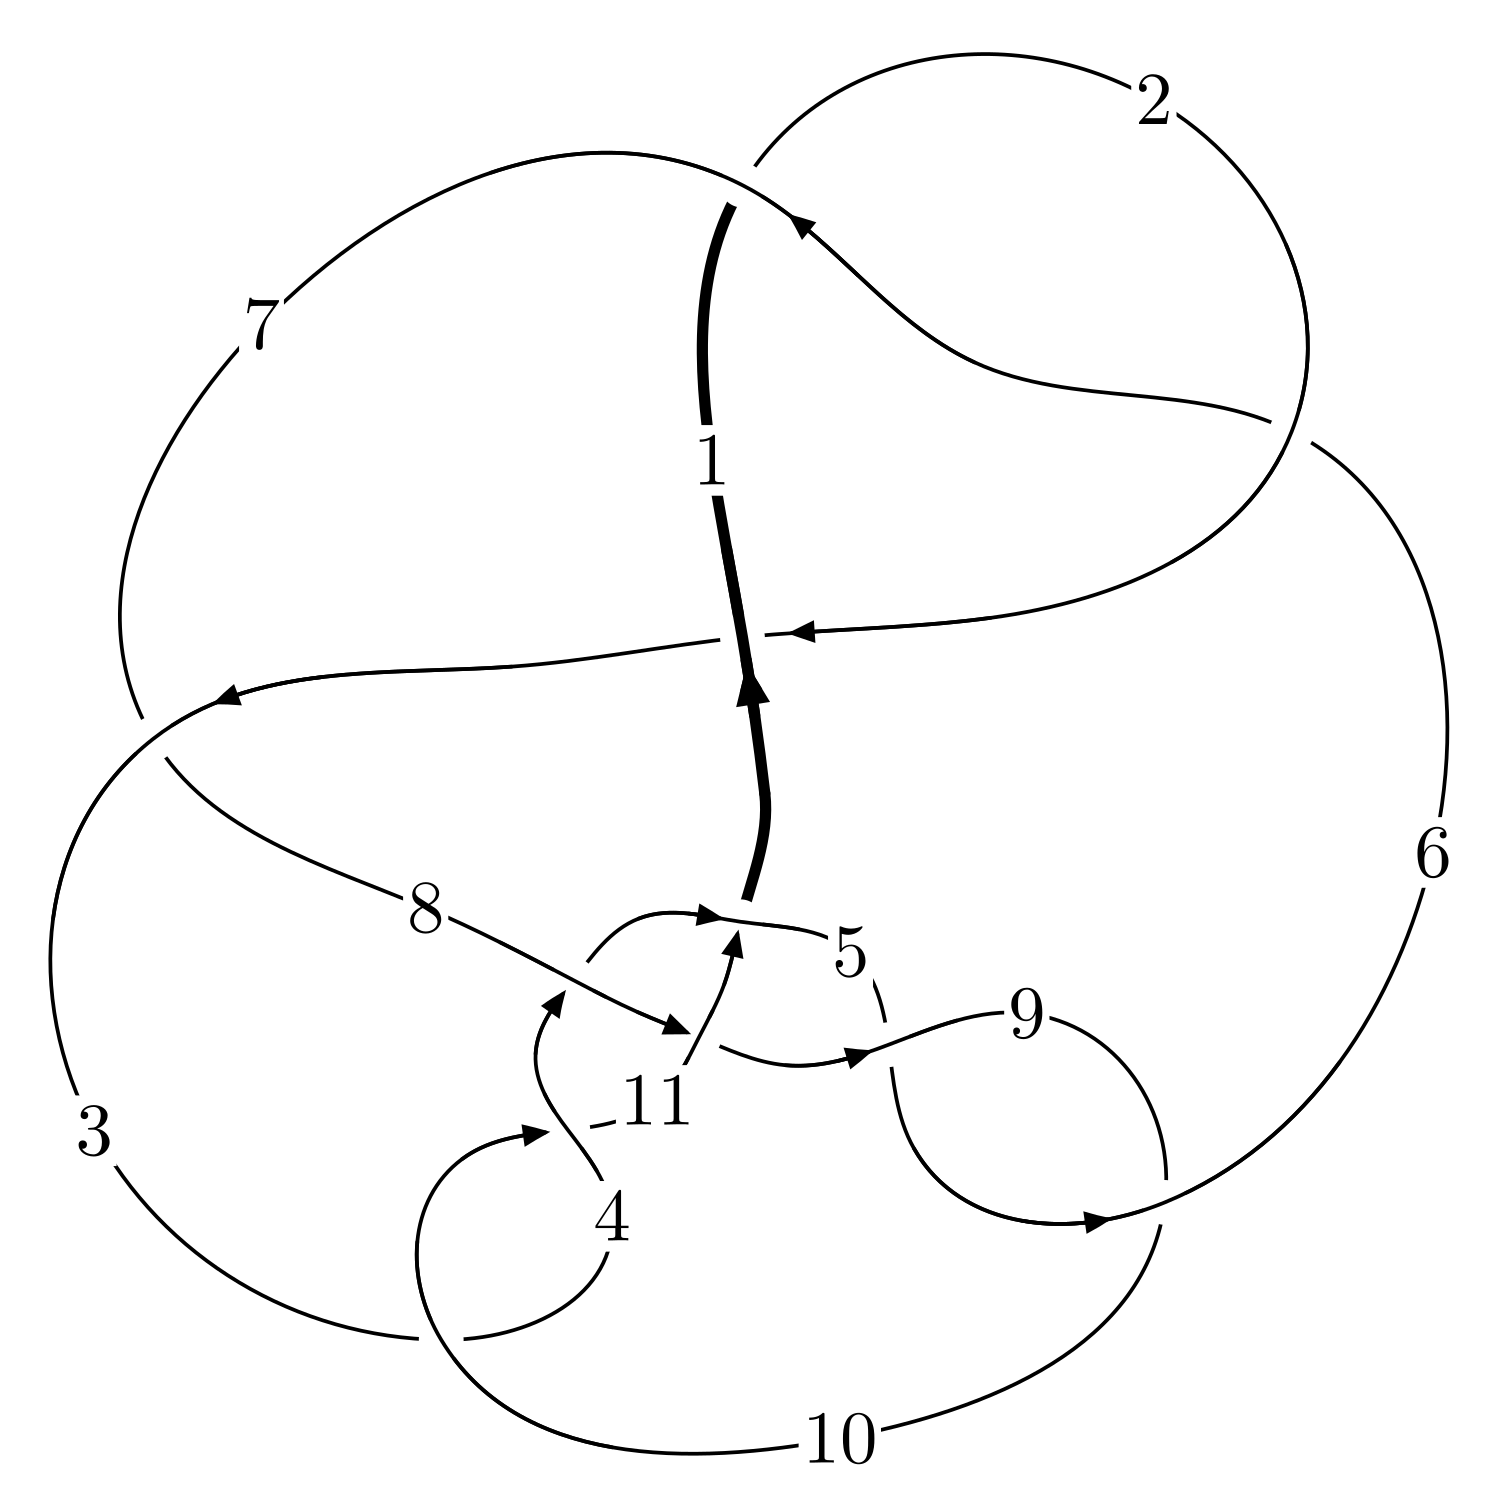
\includegraphics[width=112pt]{../../../GIT/diagram.site/Diagrams/png/445_11a_196.png}\\
\ \ \ A knot diagram\footnotemark}&
\allowdisplaybreaks
\textbf{Linearized knot diagam} \\
\cline{2-2}
 &
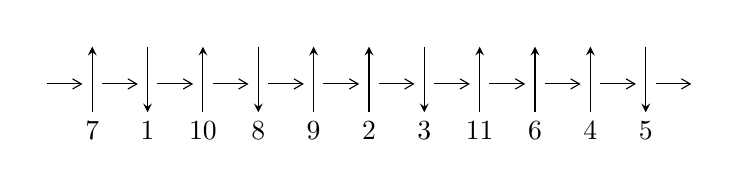
\begin{tikzpicture}[x=20pt, y=17pt]
	% nodes
	\node (C0) at (0, 0) {};
	\node (C1) at (1, 0) {};
	\node (C1U) at (1, +1) {};
	\node (C1D) at (1, -1) {7};

	\node (C2) at (2, 0) {};
	\node (C2U) at (2, +1) {};
	\node (C2D) at (2, -1) {1};

	\node (C3) at (3, 0) {};
	\node (C3U) at (3, +1) {};
	\node (C3D) at (3, -1) {10};

	\node (C4) at (4, 0) {};
	\node (C4U) at (4, +1) {};
	\node (C4D) at (4, -1) {8};

	\node (C5) at (5, 0) {};
	\node (C5U) at (5, +1) {};
	\node (C5D) at (5, -1) {9};

	\node (C6) at (6, 0) {};
	\node (C6U) at (6, +1) {};
	\node (C6D) at (6, -1) {2};

	\node (C7) at (7, 0) {};
	\node (C7U) at (7, +1) {};
	\node (C7D) at (7, -1) {3};

	\node (C8) at (8, 0) {};
	\node (C8U) at (8, +1) {};
	\node (C8D) at (8, -1) {11};

	\node (C9) at (9, 0) {};
	\node (C9U) at (9, +1) {};
	\node (C9D) at (9, -1) {6};

	\node (C10) at (10, 0) {};
	\node (C10U) at (10, +1) {};
	\node (C10D) at (10, -1) {4};

	\node (C11) at (11, 0) {};
	\node (C11U) at (11, +1) {};
	\node (C11D) at (11, -1) {5};
	\node (C12) at (12, 0) {};

	% arrows
	\draw[->,>={angle 60}]
	(C0) edge (C1) (C1) edge (C2) (C2) edge (C3) (C3) edge (C4) (C4) edge (C5) (C5) edge (C6) (C6) edge (C7) (C7) edge (C8) (C8) edge (C9) (C9) edge (C10) (C10) edge (C11) (C11) edge (C12) ;	\draw[->,>=stealth]
	(C1D) edge (C1U) (C2U) edge (C2D) (C3D) edge (C3U) (C4U) edge (C4D) (C5D) edge (C5U) (C6D) edge (C6U) (C7U) edge (C7D) (C8D) edge (C8U) (C9D) edge (C9U) (C10D) edge (C10U) (C11U) edge (C11D) ;
	\end{tikzpicture} \\
\hhline{~~} \\& 
\textbf{Solving Sequence} \\ \cline{2-2} 
 &
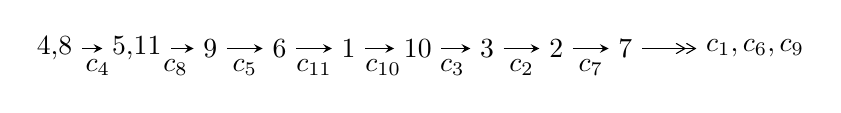
\begin{tikzpicture}[x=25pt, y=7pt]
	% node
	\node (A0) at (-1/8, 0) {4,8};
	\node (A1) at (17/16, 0) {5,11};
	\node (A2) at (17/8, 0) {9};
	\node (A3) at (25/8, 0) {6};
	\node (A4) at (33/8, 0) {1};
	\node (A5) at (41/8, 0) {10};
	\node (A6) at (49/8, 0) {3};
	\node (A7) at (57/8, 0) {2};
	\node (A8) at (65/8, 0) {7};
	\node (C1) at (1/2, -1) {$c_{4}$};
	\node (C2) at (13/8, -1) {$c_{8}$};
	\node (C3) at (21/8, -1) {$c_{5}$};
	\node (C4) at (29/8, -1) {$c_{11}$};
	\node (C5) at (37/8, -1) {$c_{10}$};
	\node (C6) at (45/8, -1) {$c_{3}$};
	\node (C7) at (53/8, -1) {$c_{2}$};
	\node (C8) at (61/8, -1) {$c_{7}$};
	\node (A9) at (10, 0) {$c_{1},c_{6},c_{9}$};

	% edge
	\draw[->,>=stealth]	
	(A0) edge (A1) (A1) edge (A2) (A2) edge (A3) (A3) edge (A4) (A4) edge (A5) (A5) edge (A6) (A6) edge (A7) (A7) edge (A8) ;
	\draw[->>,>={angle 60}]	
	(A8) edge (A9);
\end{tikzpicture} \\ 

\end{tabular} \\

\footnotetext{
The image of knot diagram is generated by the software ``\textbf{Draw programme}" developed by Andrew Bartholomew(\url{http://www.layer8.co.uk/maths/draw/index.htm\#Running-draw}), where we modified some parts for our purpose(\url{https://github.com/CATsTAILs/LinksPainter}).
}\phantom \\ \newline 
\centering \textbf{Ideals for irreducible components\footnotemark of $X_{\text{par}}$} 
 
\begin{align*}
I^u_{1}&=\langle 
-1.56366\times10^{21} u^{26}+2.00582\times10^{21} u^{25}+\cdots+7.42142\times10^{21} b-9.93961\times10^{20},\\
\phantom{I^u_{1}}&\phantom{= \langle  }-1.23252\times10^{22} u^{26}+1.13313\times10^{22} u^{25}+\cdots+7.42142\times10^{21} a-2.69156\times10^{22},\;u^{27}- u^{26}+\cdots+2 u-1\rangle \\
I^u_{2}&=\langle 
-466470675905338 u^{23}-397267180404293 u^{22}+\cdots+6630830886537376 b-264157828925488,\\
\phantom{I^u_{2}}&\phantom{= \langle  }26944089879716 u^{23}+14049375398024 u^{22}+\cdots+121666621771328 a-16982188896888,\\
\phantom{I^u_{2}}&\phantom{= \langle  }u^{24}+3 u^{22}+\cdots-4 u+8\rangle \\
I^u_{3}&=\langle 
u^{14}-3 u^{10}- u^9-2 u^8- u^7+3 u^6+4 u^5+4 u^4+u^3- u^2+2 b-3,\\
\phantom{I^u_{3}}&\phantom{= \langle  }-2 u^{14}-3 u^{13}- u^{12}-5 u^{11}+u^{10}+6 u^9+u^8+13 u^7+6 u^6-7 u^5+u^4-7 u^3-8 u^2+2 a+u-1,\\
\phantom{I^u_{3}}&\phantom{= \langle  }u^{15}+u^{13}+u^{12}-2 u^{11}-2 u^9-4 u^8+2 u^7+u^5+4 u^4-1\rangle \\
I^u_{4}&=\langle 
5.79410\times10^{18} u^{23}+1.97168\times10^{19} u^{22}+\cdots+1.42067\times10^{19} b-3.77005\times10^{17},\\
\phantom{I^u_{4}}&\phantom{= \langle  }19264503378333 u^{23}+64217498098488 u^{22}+\cdots+8090899806416 a-59730846409593,\\
\phantom{I^u_{4}}&\phantom{= \langle  }u^{24}+3 u^{23}+\cdots-6 u+1\rangle \\
I^u_{5}&=\langle 
b-1,\;59 u^5+76 u^4+242 u^3+190 u^2+67 a+487 u+146,\;u^6+u^5+4 u^4+2 u^3+8 u^2+1\rangle \\
I^u_{6}&=\langle 
- u^2+b,\;- u^2+a-1,\;u^6- u^5+2 u^4-2 u^3+2 u^2-2 u+1\rangle \\
I^u_{7}&=\langle 
b-1,\;a-2,\;u+1\rangle \\
\\
\end{align*}
\raggedright * 7 irreducible components of $\dim_{\mathbb{C}}=0$, with total 103 representations.\\
\footnotetext{All coefficients of polynomials are rational numbers. But the coefficients are sometimes approximated in decimal forms when there is not enough margin.}
\newpage
\renewcommand{\arraystretch}{1}
\centering \section*{I. $I^u_{1}= \langle -1.56\times10^{21} u^{26}+2.01\times10^{21} u^{25}+\cdots+7.42\times10^{21} b-9.94\times10^{20},\;-1.23\times10^{22} u^{26}+1.13\times10^{22} u^{25}+\cdots+7.42\times10^{21} a-2.69\times10^{22},\;u^{27}- u^{26}+\cdots+2 u-1 \rangle$}
\flushleft \textbf{(i) Arc colorings}\\
\begin{tabular}{m{7pt} m{180pt} m{7pt} m{180pt} }
\flushright $a_{4}=$&$\begin{pmatrix}1\\0\end{pmatrix}$ \\
\flushright $a_{8}=$&$\begin{pmatrix}0\\u\end{pmatrix}$ \\
\flushright $a_{5}=$&$\begin{pmatrix}1\\u^2\end{pmatrix}$ \\
\flushright $a_{11}=$&$\begin{pmatrix}1.66077 u^{26}-1.52684 u^{25}+\cdots+1.11901 u+3.62674\\0.210696 u^{26}-0.270275 u^{25}+\cdots+2.39290 u+0.133931\end{pmatrix}$ \\
\flushright $a_{9}=$&$\begin{pmatrix}0.312172 u^{26}+0.638396 u^{25}+\cdots-1.77480 u+3.01621\\0.581257 u^{26}-0.629489 u^{25}+\cdots+0.803940 u+1.08450\end{pmatrix}$ \\
\flushright $a_{6}=$&$\begin{pmatrix}-1.18988 u^{26}+1.11302 u^{25}+\cdots-4.45598 u+1.89491\\-0.241743 u^{26}+0.0536668 u^{25}+\cdots-0.670686 u-0.868814\end{pmatrix}$ \\
\flushright $a_{1}=$&$\begin{pmatrix}1.66077 u^{26}-1.52684 u^{25}+\cdots+0.119008 u+3.62674\\0.210696 u^{26}-0.270275 u^{25}+\cdots+2.39290 u+0.133931\end{pmatrix}$ \\
\flushright $a_{10}=$&$\begin{pmatrix}1.45007 u^{26}-1.25656 u^{25}+\cdots-1.27390 u+3.49281\\0.210696 u^{26}-0.270275 u^{25}+\cdots+2.39290 u+0.133931\end{pmatrix}$ \\
\flushright $a_{3}=$&$\begin{pmatrix}1.19231 u^{26}-0.633674 u^{25}+\cdots+3.06255 u+2.18099\\-0.107812 u^{26}+0.130431 u^{25}+\cdots-0.365474 u+0.791952\end{pmatrix}$ \\
\flushright $a_{2}=$&$\begin{pmatrix}1.19260 u^{26}-0.799146 u^{25}+\cdots+2.64209 u-0.651268\\-0.0394366 u^{26}+0.164653 u^{25}+\cdots+0.0481946 u+0.646177\end{pmatrix}$ \\
\flushright $a_{7}=$&$\begin{pmatrix}-0.451600 u^{26}+0.986823 u^{25}+\cdots+5.66786 u-0.00121263\\0.328533 u^{26}-0.284050 u^{25}+\cdots-0.908870 u+0.936550\end{pmatrix}$\\ \flushright $a_{7}=$&$\begin{pmatrix}-0.451600 u^{26}+0.986823 u^{25}+\cdots+5.66786 u-0.00121263\\0.328533 u^{26}-0.284050 u^{25}+\cdots-0.908870 u+0.936550\end{pmatrix}$\\&\end{tabular}
\flushleft \textbf{(ii) Obstruction class $= -1$}\\~\\
\flushleft \textbf{(iii) Cusp Shapes $= \frac{24366089866600657610153}{7421416129906443651586} u^{26}-\frac{13344042961471974440973}{3710708064953221825793} u^{25}+\cdots+\frac{123365016888052989817509}{7421416129906443651586} u+\frac{5771013155102072120085}{3710708064953221825793}$}\\~\\
\newpage\renewcommand{\arraystretch}{1}
\flushleft \textbf{(iv) u-Polynomials at the component}\newline \\
\begin{tabular}{m{50pt}|m{274pt}}
Crossings & \hspace{64pt}u-Polynomials at each crossing \\
\hline $$\begin{aligned}c_{1},c_{6}\end{aligned}$$&$\begin{aligned}
&u^{27}+6 u^{26}+\cdots-40 u-8
\end{aligned}$\\
\hline $$\begin{aligned}c_{2}\end{aligned}$$&$\begin{aligned}
&u^{27}+14 u^{26}+\cdots+32 u-64
\end{aligned}$\\
\hline $$\begin{aligned}c_{3},c_{5},c_{9}\\c_{10}\end{aligned}$$&$\begin{aligned}
&u^{27}-9 u^{25}+\cdots- u-1
\end{aligned}$\\
\hline $$\begin{aligned}c_{4},c_{11}\end{aligned}$$&$\begin{aligned}
&u^{27}- u^{26}+\cdots+2 u-1
\end{aligned}$\\
\hline $$\begin{aligned}c_{7}\end{aligned}$$&$\begin{aligned}
&u^{27}-9 u^{26}+\cdots+2296 u-232
\end{aligned}$\\
\hline $$\begin{aligned}c_{8}\end{aligned}$$&$\begin{aligned}
&u^{27}+22 u^{26}+\cdots-7680 u-512
\end{aligned}$\\
\hline
\end{tabular}\\~\\
\newpage\renewcommand{\arraystretch}{1}
\flushleft \textbf{(v) Riley Polynomials at the component}\newline \\
\begin{tabular}{m{50pt}|m{274pt}}
Crossings & \hspace{64pt}Riley Polynomials at each crossing \\
\hline $$\begin{aligned}c_{1},c_{6}\end{aligned}$$&$\begin{aligned}
&y^{27}+14 y^{26}+\cdots+32 y-64
\end{aligned}$\\
\hline $$\begin{aligned}c_{2}\end{aligned}$$&$\begin{aligned}
&y^{27}+2 y^{26}+\cdots+39424 y-4096
\end{aligned}$\\
\hline $$\begin{aligned}c_{3},c_{5},c_{9}\\c_{10}\end{aligned}$$&$\begin{aligned}
&y^{27}-18 y^{26}+\cdots-7 y-1
\end{aligned}$\\
\hline $$\begin{aligned}c_{4},c_{11}\end{aligned}$$&$\begin{aligned}
&y^{27}-5 y^{26}+\cdots+16 y-1
\end{aligned}$\\
\hline $$\begin{aligned}c_{7}\end{aligned}$$&$\begin{aligned}
&y^{27}-7 y^{26}+\cdots+586144 y-53824
\end{aligned}$\\
\hline $$\begin{aligned}c_{8}\end{aligned}$$&$\begin{aligned}
&y^{27}-4 y^{26}+\cdots+1966080 y-262144
\end{aligned}$\\
\hline
\end{tabular}\\~\\
\newpage\flushleft \textbf{(vi) Complex Volumes and Cusp Shapes}
$$\begin{array}{c|c|c}  
\text{Solutions to }I^u_{1}& \I (\text{vol} + \sqrt{-1}CS) & \text{Cusp shape}\\
 \hline 
\begin{aligned}
u &= -0.898231 + 0.526385 I \\
a &= \phantom{-}0.209642 + 0.703154 I \\
b &= -0.122251 + 0.700628 I\end{aligned}
 & -1.84219 + 1.61763 I & -0.34752 - 1.90846 I \\ \hline\begin{aligned}
u &= -0.898231 - 0.526385 I \\
a &= \phantom{-}0.209642 - 0.703154 I \\
b &= -0.122251 - 0.700628 I\end{aligned}
 & -1.84219 - 1.61763 I & -0.34752 + 1.90846 I \\ \hline\begin{aligned}
u &= \phantom{-}1.012540 + 0.318884 I \\
a &= -0.308945 + 0.757476 I \\
b &= \phantom{-}0.238061 + 0.818947 I\end{aligned}
 & -5.36570 + 2.03204 I & -4.32275 - 2.13513 I \\ \hline\begin{aligned}
u &= \phantom{-}1.012540 - 0.318884 I \\
a &= -0.308945 - 0.757476 I \\
b &= \phantom{-}0.238061 - 0.818947 I\end{aligned}
 & -5.36570 - 2.03204 I & -4.32275 + 2.13513 I \\ \hline\begin{aligned}
u &= -0.276412 + 0.776716 I \\
a &= \phantom{-}0.023671 + 0.586360 I \\
b &= -0.037108 + 0.457608 I\end{aligned}
 & \phantom{-}0.18488 + 1.81939 I & \phantom{-}2.29374 - 3.76762 I \\ \hline\begin{aligned}
u &= -0.276412 - 0.776716 I \\
a &= \phantom{-}0.023671 - 0.586360 I \\
b &= -0.037108 - 0.457608 I\end{aligned}
 & \phantom{-}0.18488 - 1.81939 I & \phantom{-}2.29374 + 3.76762 I \\ \hline\begin{aligned}
u &= -0.795815 + 0.903407 I \\
a &= \phantom{-}0.26309 + 1.49507 I \\
b &= \phantom{-}1.305830 + 0.251781 I\end{aligned}
 & \phantom{-}7.97470 + 2.85426 I & \phantom{-}8.94272 - 2.79876 I \\ \hline\begin{aligned}
u &= -0.795815 - 0.903407 I \\
a &= \phantom{-}0.26309 - 1.49507 I \\
b &= \phantom{-}1.305830 - 0.251781 I\end{aligned}
 & \phantom{-}7.97470 - 2.85426 I & \phantom{-}8.94272 + 2.79876 I \\ \hline\begin{aligned}
u &= \phantom{-}1.074420 + 0.604846 I \\
a &= -0.257278 + 0.648739 I \\
b &= \phantom{-}0.028367 + 0.782017 I\end{aligned}
 & -4.76097 - 6.00409 I & -3.69772 + 5.84582 I \\ \hline\begin{aligned}
u &= \phantom{-}1.074420 - 0.604846 I \\
a &= -0.257278 - 0.648739 I \\
b &= \phantom{-}0.028367 - 0.782017 I\end{aligned}
 & -4.76097 + 6.00409 I & -3.69772 - 5.84582 I\\
 \hline 
 \end{array}$$\newpage$$\begin{array}{c|c|c}  
\text{Solutions to }I^u_{1}& \I (\text{vol} + \sqrt{-1}CS) & \text{Cusp shape}\\
 \hline 
\begin{aligned}
u &= \phantom{-}1.208550 + 0.274221 I \\
a &= -1.302050 + 0.508274 I \\
b &= -0.932187 + 0.115358 I\end{aligned}
 & -2.56542 - 5.05729 I & \phantom{-}5.23613 + 5.90187 I \\ \hline\begin{aligned}
u &= \phantom{-}1.208550 - 0.274221 I \\
a &= -1.302050 - 0.508274 I \\
b &= -0.932187 - 0.115358 I\end{aligned}
 & -2.56542 + 5.05729 I & \phantom{-}5.23613 - 5.90187 I \\ \hline\begin{aligned}
u &= \phantom{-}0.878818 + 1.037850 I \\
a &= -0.167256 + 1.255180 I \\
b &= -1.359850 + 0.350164 I\end{aligned}
 & \phantom{-}8.49644 - 8.55345 I & \phantom{-}9.20145 + 7.26296 I \\ \hline\begin{aligned}
u &= \phantom{-}0.878818 - 1.037850 I \\
a &= -0.167256 - 1.255180 I \\
b &= -1.359850 - 0.350164 I\end{aligned}
 & \phantom{-}8.49644 + 8.55345 I & \phantom{-}9.20145 - 7.26296 I \\ \hline\begin{aligned}
u &= -0.421872 + 0.462971 I \\
a &= \phantom{-}2.45358 - 1.32260 I \\
b &= -1.027750 - 0.447368 I\end{aligned}
 & \phantom{-}0.99303 + 9.06795 I & \phantom{-}3.46736 - 11.63407 I \\ \hline\begin{aligned}
u &= -0.421872 - 0.462971 I \\
a &= \phantom{-}2.45358 + 1.32260 I \\
b &= -1.027750 + 0.447368 I\end{aligned}
 & \phantom{-}0.99303 - 9.06795 I & \phantom{-}3.46736 + 11.63407 I \\ \hline\begin{aligned}
u &= -0.591031 + 0.138214 I \\
a &= \phantom{-}0.54492 - 1.69705 I \\
b &= -0.688350 - 0.511205 I\end{aligned}
 & -2.72477 + 1.50676 I & -3.17250 - 4.01509 I \\ \hline\begin{aligned}
u &= -0.591031 - 0.138214 I \\
a &= \phantom{-}0.54492 + 1.69705 I \\
b &= -0.688350 + 0.511205 I\end{aligned}
 & -2.72477 - 1.50676 I & -3.17250 + 4.01509 I \\ \hline\begin{aligned}
u &= \phantom{-}0.338852 + 0.350615 I \\
a &= -3.02283 - 2.53673 I \\
b &= \phantom{-}0.966126 - 0.347074 I\end{aligned}
 & \phantom{-}3.01066 - 3.39049 I & \phantom{-}3.02884 + 10.08685 I \\ \hline\begin{aligned}
u &= \phantom{-}0.338852 - 0.350615 I \\
a &= -3.02283 + 2.53673 I \\
b &= \phantom{-}0.966126 + 0.347074 I\end{aligned}
 & \phantom{-}3.01066 + 3.39049 I & \phantom{-}3.02884 - 10.08685 I\\
 \hline 
 \end{array}$$\newpage$$\begin{array}{c|c|c}  
\text{Solutions to }I^u_{1}& \I (\text{vol} + \sqrt{-1}CS) & \text{Cusp shape}\\
 \hline 
\begin{aligned}
u &= -1.13972 + 1.08957 I \\
a &= \phantom{-}0.255186 + 0.962671 I \\
b &= \phantom{-}1.279710 + 0.563405 I\end{aligned}
 & \phantom{-}0.91508 + 8.68990 I & \phantom{-}2.54049 - 5.35859 I \\ \hline\begin{aligned}
u &= -1.13972 - 1.08957 I \\
a &= \phantom{-}0.255186 - 0.962671 I \\
b &= \phantom{-}1.279710 - 0.563405 I\end{aligned}
 & \phantom{-}0.91508 - 8.68990 I & \phantom{-}2.54049 + 5.35859 I \\ \hline\begin{aligned}
u &= \phantom{-}1.07737 + 1.19752 I \\
a &= -0.142409 + 0.974746 I \\
b &= -1.39888 + 0.56362 I\end{aligned}
 & \phantom{-}6.16613 - 11.88750 I & \phantom{-}7.81516 + 6.29925 I \\ \hline\begin{aligned}
u &= \phantom{-}1.07737 - 1.19752 I \\
a &= -0.142409 - 0.974746 I \\
b &= -1.39888 - 0.56362 I\end{aligned}
 & \phantom{-}6.16613 + 11.88750 I & \phantom{-}7.81516 - 6.29925 I \\ \hline\begin{aligned}
u &= -1.12228 + 1.24272 I \\
a &= \phantom{-}0.128320 + 0.924082 I \\
b &= \phantom{-}1.41876 + 0.62158 I\end{aligned}
 & \phantom{-}3.6775 + 17.2855 I & \phantom{-}4.85544 - 9.87335 I \\ \hline\begin{aligned}
u &= -1.12228 - 1.24272 I \\
a &= \phantom{-}0.128320 - 0.924082 I \\
b &= \phantom{-}1.41876 - 0.62158 I\end{aligned}
 & \phantom{-}3.6775 - 17.2855 I & \phantom{-}4.85544 + 9.87335 I \\ \hline\begin{aligned}
u &= \phantom{-}0.309622\phantom{ +0.000000I} \\
a &= \phantom{-}3.64471\phantom{ +0.000000I} \\
b &= \phantom{-}0.659027\phantom{ +0.000000I}\end{aligned}
 & \phantom{-}1.29009\phantom{ +0.000000I} & \phantom{-}9.31830\phantom{ +0.000000I}\\
 \hline 
 \end{array}$$\newpage\newpage\renewcommand{\arraystretch}{1}
\centering \section*{II. $I^u_{2}= \langle -4.66\times10^{14} u^{23}-3.97\times10^{14} u^{22}+\cdots+6.63\times10^{15} b-2.64\times10^{14},\;2.69\times10^{13} u^{23}+1.40\times10^{13} u^{22}+\cdots+1.22\times10^{14} a-1.70\times10^{13},\;u^{24}+3 u^{22}+\cdots-4 u+8 \rangle$}
\flushleft \textbf{(i) Arc colorings}\\
\begin{tabular}{m{7pt} m{180pt} m{7pt} m{180pt} }
\flushright $a_{4}=$&$\begin{pmatrix}1\\0\end{pmatrix}$ \\
\flushright $a_{8}=$&$\begin{pmatrix}0\\u\end{pmatrix}$ \\
\flushright $a_{5}=$&$\begin{pmatrix}1\\u^2\end{pmatrix}$ \\
\flushright $a_{11}=$&$\begin{pmatrix}-0.221458 u^{23}-0.115474 u^{22}+\cdots-5.16359 u+0.139580\\0.0703488 u^{23}+0.0599121 u^{22}+\cdots+3.44503 u+0.0398378\end{pmatrix}$ \\
\flushright $a_{9}=$&$\begin{pmatrix}-0.131260 u^{23}-0.121483 u^{22}+\cdots-3.05755 u+2.19329\\-0.0922969 u^{23}+0.000104233 u^{22}+\cdots-1.11867 u-0.780159\end{pmatrix}$ \\
\flushright $a_{6}=$&$\begin{pmatrix}-0.108244 u^{23}+0.149259 u^{22}+\cdots+1.62669 u+5.33342\\0.00600815 u^{23}+0.116833 u^{22}+\cdots-2.41450 u-0.278416\end{pmatrix}$ \\
\flushright $a_{1}=$&$\begin{pmatrix}-0.277967 u^{23}-0.143397 u^{22}+\cdots-7.29884 u+1.02354\\0.0235493 u^{23}+0.106410 u^{22}+\cdots+3.78541 u+0.263215\end{pmatrix}$ \\
\flushright $a_{10}=$&$\begin{pmatrix}-0.291807 u^{23}-0.175386 u^{22}+\cdots-8.60861 u+0.0997419\\0.0703488 u^{23}+0.0599121 u^{22}+\cdots+3.44503 u+0.0398378\end{pmatrix}$ \\
\flushright $a_{3}=$&$\begin{pmatrix}0.187834 u^{23}+0.00949931 u^{22}+\cdots+7.51428 u-1.76112\\-0.0903139 u^{23}-0.101796 u^{22}+\cdots+0.0682743 u+0.252378\end{pmatrix}$ \\
\flushright $a_{2}=$&$\begin{pmatrix}-0.0733779 u^{23}+0.0153619 u^{22}+\cdots+9.34212 u+4.09583\\0.123742 u^{23}-0.0875102 u^{22}+\cdots-0.0211572 u-1.70617\end{pmatrix}$ \\
\flushright $a_{7}=$&$\begin{pmatrix}-0.340801 u^{23}-0.152896 u^{22}+\cdots-7.31312 u+2.28466\\0.170602 u^{23}+0.00657076 u^{22}+\cdots+1.79380 u-0.738436\end{pmatrix}$\\ \flushright $a_{7}=$&$\begin{pmatrix}-0.340801 u^{23}-0.152896 u^{22}+\cdots-7.31312 u+2.28466\\0.170602 u^{23}+0.00657076 u^{22}+\cdots+1.79380 u-0.738436\end{pmatrix}$\\&\end{tabular}
\flushleft \textbf{(ii) Obstruction class $= -1$}\\~\\
\flushleft \textbf{(iii) Cusp Shapes $= \frac{867553217111521}{1657707721634344} u^{23}+\frac{56390307623253}{3315415443268688} u^{22}+\cdots+\frac{3770100918086014}{207213465204293} u+\frac{1919092137145043}{207213465204293}$}\\~\\
\newpage\renewcommand{\arraystretch}{1}
\flushleft \textbf{(iv) u-Polynomials at the component}\newline \\
\begin{tabular}{m{50pt}|m{274pt}}
Crossings & \hspace{64pt}u-Polynomials at each crossing \\
\hline $$\begin{aligned}c_{1},c_{6}\end{aligned}$$&$\begin{aligned}
&(u^4+u^2+u+1)^6
\end{aligned}$\\
\hline $$\begin{aligned}c_{2}\end{aligned}$$&$\begin{aligned}
&(u^4+2 u^3+3 u^2+u+1)^6
\end{aligned}$\\
\hline $$\begin{aligned}c_{3},c_{5},c_{9}\\c_{10}\end{aligned}$$&$\begin{aligned}
&u^{24}-9 u^{22}+\cdots+56 u+8
\end{aligned}$\\
\hline $$\begin{aligned}c_{4},c_{11}\end{aligned}$$&$\begin{aligned}
&u^{24}+3 u^{22}+\cdots-4 u+8
\end{aligned}$\\
\hline $$\begin{aligned}c_{7}\end{aligned}$$&$\begin{aligned}
&(u^4+3 u^3+4 u^2+3 u+2)^6
\end{aligned}$\\
\hline $$\begin{aligned}c_{8}\end{aligned}$$&$\begin{aligned}
&(u^3- u^2+1)^8
\end{aligned}$\\
\hline
\end{tabular}\\~\\
\newpage\renewcommand{\arraystretch}{1}
\flushleft \textbf{(v) Riley Polynomials at the component}\newline \\
\begin{tabular}{m{50pt}|m{274pt}}
Crossings & \hspace{64pt}Riley Polynomials at each crossing \\
\hline $$\begin{aligned}c_{1},c_{6}\end{aligned}$$&$\begin{aligned}
&(y^4+2 y^3+3 y^2+y+1)^6
\end{aligned}$\\
\hline $$\begin{aligned}c_{2}\end{aligned}$$&$\begin{aligned}
&(y^4+2 y^3+7 y^2+5 y+1)^6
\end{aligned}$\\
\hline $$\begin{aligned}c_{3},c_{5},c_{9}\\c_{10}\end{aligned}$$&$\begin{aligned}
&y^{24}-18 y^{23}+\cdots-864 y+64
\end{aligned}$\\
\hline $$\begin{aligned}c_{4},c_{11}\end{aligned}$$&$\begin{aligned}
&y^{24}+6 y^{23}+\cdots+944 y+64
\end{aligned}$\\
\hline $$\begin{aligned}c_{7}\end{aligned}$$&$\begin{aligned}
&(y^4- y^3+2 y^2+7 y+4)^6
\end{aligned}$\\
\hline $$\begin{aligned}c_{8}\end{aligned}$$&$\begin{aligned}
&(y^3- y^2+2 y-1)^8
\end{aligned}$\\
\hline
\end{tabular}\\~\\
\newpage\flushleft \textbf{(vi) Complex Volumes and Cusp Shapes}
$$\begin{array}{c|c|c}  
\text{Solutions to }I^u_{2}& \I (\text{vol} + \sqrt{-1}CS) & \text{Cusp shape}\\
 \hline 
\begin{aligned}
u &= \phantom{-}0.077838 + 1.001210 I \\
a &= -0.058264 + 0.749436 I \\
b &= -1.40920 + 0.84871 I\end{aligned}
 & \phantom{-}3.42323 - 7.64338 I & \phantom{-}9.24932 + 6.51087 I \\ \hline\begin{aligned}
u &= \phantom{-}0.077838 - 1.001210 I \\
a &= -0.058264 - 0.749436 I \\
b &= -1.40920 - 0.84871 I\end{aligned}
 & \phantom{-}3.42323 + 7.64338 I & \phantom{-}9.24932 - 6.51087 I \\ \hline\begin{aligned}
u &= \phantom{-}0.554955 + 0.881319 I \\
a &= -0.156285 - 1.094010 I \\
b &= \phantom{-}0.443978 - 1.026930 I\end{aligned}
 & \phantom{-}2.89077 - 4.22521 I & \phantom{-}8.26043 + 6.84681 I \\ \hline\begin{aligned}
u &= \phantom{-}0.554955 - 0.881319 I \\
a &= -0.156285 + 1.094010 I \\
b &= \phantom{-}0.443978 + 1.026930 I\end{aligned}
 & \phantom{-}2.89077 + 4.22521 I & \phantom{-}8.26043 - 6.84681 I \\ \hline\begin{aligned}
u &= \phantom{-}0.214202 + 0.934183 I \\
a &= \phantom{-}0.962122 - 0.718649 I \\
b &= -0.207958 + 0.155122 I\end{aligned}
 & \phantom{-}2.89077 + 1.43103 I & \phantom{-}8.26043 + 0.88791 I \\ \hline\begin{aligned}
u &= \phantom{-}0.214202 - 0.934183 I \\
a &= \phantom{-}0.962122 + 0.718649 I \\
b &= -0.207958 - 0.155122 I\end{aligned}
 & \phantom{-}2.89077 - 1.43103 I & \phantom{-}8.26043 - 0.88791 I \\ \hline\begin{aligned}
u &= -0.810739 + 0.684928 I \\
a &= -0.178616 - 1.069640 I \\
b &= \phantom{-}0.034600 - 1.374090 I\end{aligned}
 & -0.71436 + 10.47150 I & \phantom{-}2.72006 - 9.49032 I \\ \hline\begin{aligned}
u &= -0.810739 - 0.684928 I \\
a &= -0.178616 + 1.069640 I \\
b &= \phantom{-}0.034600 + 1.374090 I\end{aligned}
 & -0.71436 - 10.47150 I & \phantom{-}2.72006 + 9.49032 I \\ \hline\begin{aligned}
u &= -1.023630 + 0.332750 I \\
a &= -0.989201 + 0.406110 I \\
b &= -0.441767 + 0.651030 I\end{aligned}
 & -0.71436 + 4.81525 I & \phantom{-}2.72006 - 3.53142 I \\ \hline\begin{aligned}
u &= -1.023630 - 0.332750 I \\
a &= -0.989201 - 0.406110 I \\
b &= -0.441767 - 0.651030 I\end{aligned}
 & -0.71436 - 4.81525 I & \phantom{-}2.72006 + 3.53142 I\\
 \hline 
 \end{array}$$\newpage$$\begin{array}{c|c|c}  
\text{Solutions to }I^u_{2}& \I (\text{vol} + \sqrt{-1}CS) & \text{Cusp shape}\\
 \hline 
\begin{aligned}
u &= \phantom{-}0.299931 + 0.824118 I \\
a &= -0.455949 - 1.230640 I \\
b &= \phantom{-}1.091230 - 0.434477 I\end{aligned}
 & \phantom{-}2.89077 - 1.43103 I & \phantom{-}8.26043 - 0.88791 I \\ \hline\begin{aligned}
u &= \phantom{-}0.299931 - 0.824118 I \\
a &= -0.455949 + 1.230640 I \\
b &= \phantom{-}1.091230 + 0.434477 I\end{aligned}
 & \phantom{-}2.89077 + 1.43103 I & \phantom{-}8.26043 + 0.88791 I \\ \hline\begin{aligned}
u &= -0.233421 + 0.551322 I \\
a &= \phantom{-}0.491584 + 1.161090 I \\
b &= \phantom{-}1.68223 + 0.39397 I\end{aligned}
 & \phantom{-}7.02835 + 1.39709 I & \phantom{-}14.7897 - 3.8674 I \\ \hline\begin{aligned}
u &= -0.233421 - 0.551322 I \\
a &= \phantom{-}0.491584 - 1.161090 I \\
b &= \phantom{-}1.68223 - 0.39397 I\end{aligned}
 & \phantom{-}7.02835 - 1.39709 I & \phantom{-}14.7897 + 3.8674 I \\ \hline\begin{aligned}
u &= \phantom{-}0.208549 + 0.403398 I \\
a &= \phantom{-}2.34438 - 0.96312 I \\
b &= -1.141110 + 0.176547 I\end{aligned}
 & -0.71436 - 4.81525 I & \phantom{-}2.72006 + 3.53142 I \\ \hline\begin{aligned}
u &= \phantom{-}0.208549 - 0.403398 I \\
a &= \phantom{-}2.34438 + 0.96312 I \\
b &= -1.141110 - 0.176547 I\end{aligned}
 & -0.71436 + 4.81525 I & \phantom{-}2.72006 - 3.53142 I \\ \hline\begin{aligned}
u &= -0.69942 + 1.38686 I \\
a &= \phantom{-}0.173806 - 0.720332 I \\
b &= -1.091770 - 0.185403 I\end{aligned}
 & \phantom{-}2.89077 + 4.22521 I & \phantom{-}8.26043 - 6.84681 I \\ \hline\begin{aligned}
u &= -0.69942 - 1.38686 I \\
a &= \phantom{-}0.173806 + 0.720332 I \\
b &= -1.091770 + 0.185403 I\end{aligned}
 & \phantom{-}2.89077 - 4.22521 I & \phantom{-}8.26043 + 6.84681 I \\ \hline\begin{aligned}
u &= \phantom{-}1.50603 + 0.81015 I \\
a &= -0.388743 + 0.209121 I \\
b &= -1.370290 - 0.060244 I\end{aligned}
 & \phantom{-}7.02835 + 1.39709 I & \phantom{-}14.7897 - 3.8674 I \\ \hline\begin{aligned}
u &= \phantom{-}1.50603 - 0.81015 I \\
a &= -0.388743 - 0.209121 I \\
b &= -1.370290 + 0.060244 I\end{aligned}
 & \phantom{-}7.02835 - 1.39709 I & \phantom{-}14.7897 + 3.8674 I\\
 \hline 
 \end{array}$$\newpage$$\begin{array}{c|c|c}  
\text{Solutions to }I^u_{2}& \I (\text{vol} + \sqrt{-1}CS) & \text{Cusp shape}\\
 \hline 
\begin{aligned}
u &= \phantom{-}1.25615 + 1.37119 I \\
a &= \phantom{-}0.023380 - 0.618493 I \\
b &= \phantom{-}1.312800 - 0.417455 I\end{aligned}
 & -0.71436 - 10.47150 I & \phantom{-}2.72006 + 9.49032 I \\ \hline\begin{aligned}
u &= \phantom{-}1.25615 - 1.37119 I \\
a &= \phantom{-}0.023380 + 0.618493 I \\
b &= \phantom{-}1.312800 + 0.417455 I\end{aligned}
 & -0.71436 + 10.47150 I & \phantom{-}2.72006 - 9.49032 I \\ \hline\begin{aligned}
u &= -1.35044 + 1.60451 I \\
a &= \phantom{-}0.231785 + 0.275391 I \\
b &= \phantom{-}1.097260 - 0.209996 I\end{aligned}
 & \phantom{-}3.42323 - 7.64338 I & \phantom{-}9.24932 + 6.51087 I \\ \hline\begin{aligned}
u &= -1.35044 - 1.60451 I \\
a &= \phantom{-}0.231785 - 0.275391 I \\
b &= \phantom{-}1.097260 + 0.209996 I\end{aligned}
 & \phantom{-}3.42323 + 7.64338 I & \phantom{-}9.24932 - 6.51087 I\\
 \hline 
 \end{array}$$\newpage\newpage\renewcommand{\arraystretch}{1}
\centering \section*{III. $I^u_{3}= \langle u^{14}-3 u^{10}+\cdots+2 b-3,\;-2 u^{14}-3 u^{13}+\cdots+2 a-1,\;u^{15}+u^{13}+\cdots+4 u^4-1 \rangle$}
\flushleft \textbf{(i) Arc colorings}\\
\begin{tabular}{m{7pt} m{180pt} m{7pt} m{180pt} }
\flushright $a_{4}=$&$\begin{pmatrix}1\\0\end{pmatrix}$ \\
\flushright $a_{8}=$&$\begin{pmatrix}0\\u\end{pmatrix}$ \\
\flushright $a_{5}=$&$\begin{pmatrix}1\\u^2\end{pmatrix}$ \\
\flushright $a_{11}=$&$\begin{pmatrix}u^{14}+\frac{3}{2} u^{13}+\cdots-\frac{1}{2} u+\frac{1}{2}\\-\frac{1}{2} u^{14}+\frac{3}{2} u^{10}+\cdots+\frac{1}{2} u^2+\frac{3}{2}\end{pmatrix}$ \\
\flushright $a_{9}=$&$\begin{pmatrix}u^{14}+\frac{3}{2} u^{13}+\cdots+\frac{7}{2} u+\frac{1}{2}\\u^{14}+u^{12}+u^{11}-2 u^{10}-2 u^8-4 u^7+2 u^6+u^4+4 u^3+u\end{pmatrix}$ \\
\flushright $a_{6}=$&$\begin{pmatrix}\frac{1}{2} u^{14}+u^{13}+\cdots+4 u+\frac{1}{2}\\\frac{3}{2} u^{14}+2 u^{12}+\cdots+2 u-\frac{1}{2}\end{pmatrix}$ \\
\flushright $a_{1}=$&$\begin{pmatrix}u^{14}+\frac{3}{2} u^{13}+\cdots+\frac{1}{2} u+\frac{1}{2}\\-\frac{1}{2} u^{14}+\frac{3}{2} u^{10}+\cdots+\frac{1}{2} u^2+\frac{3}{2}\end{pmatrix}$ \\
\flushright $a_{10}=$&$\begin{pmatrix}\frac{3}{2} u^{14}+\frac{3}{2} u^{13}+\cdots-\frac{1}{2} u-1\\-\frac{1}{2} u^{14}+\frac{3}{2} u^{10}+\cdots+\frac{1}{2} u^2+\frac{3}{2}\end{pmatrix}$ \\
\flushright $a_{3}=$&$\begin{pmatrix}\frac{3}{2} u^{13}+\frac{1}{2} u^{12}+\cdots+\frac{3}{2} u-\frac{1}{2}\\-\frac{1}{2} u^{13}-\frac{1}{2} u^{12}+\cdots-\frac{3}{2} u+\frac{3}{2}\end{pmatrix}$ \\
\flushright $a_{2}=$&$\begin{pmatrix}- u^{14}+\frac{3}{2} u^{13}+\cdots+\frac{1}{2} u-\frac{3}{2}\\-\frac{1}{2} u^{14}- u^{13}+\cdots-2 u+\frac{3}{2}\end{pmatrix}$ \\
\flushright $a_{7}=$&$\begin{pmatrix}- u^{14}+\frac{1}{2} u^{13}+\cdots+\frac{7}{2} u+\frac{5}{2}\\2 u^{14}+2 u^{12}+\cdots+u-1\end{pmatrix}$\\ \flushright $a_{7}=$&$\begin{pmatrix}- u^{14}+\frac{1}{2} u^{13}+\cdots+\frac{7}{2} u+\frac{5}{2}\\2 u^{14}+2 u^{12}+\cdots+u-1\end{pmatrix}$\\&\end{tabular}
\flushleft \textbf{(ii) Obstruction class $= 1$}\\~\\
\flushleft \textbf{(iii) Cusp Shapes $= -\frac{11}{2} u^{14}- u^{13}-2 u^{12}-8 u^{11}+\frac{23}{2} u^{10}+\frac{7}{2} u^9+6 u^8+\frac{47}{2} u^7-\frac{9}{2} u^6-10 u^5+4 u^4-\frac{33}{2} u^3-\frac{19}{2} u^2+\frac{5}{2}$}\\~\\
\newpage\renewcommand{\arraystretch}{1}
\flushleft \textbf{(iv) u-Polynomials at the component}\newline \\
\begin{tabular}{m{50pt}|m{274pt}}
Crossings & \hspace{64pt}u-Polynomials at each crossing \\
\hline $$\begin{aligned}c_{1}\end{aligned}$$&$\begin{aligned}
&u^{15}+4 u^{13}+8 u^{11}- u^{10}+8 u^9-3 u^8+4 u^7-5 u^6-5 u^4-3 u^2-1
\end{aligned}$\\
\hline $$\begin{aligned}c_{2}\end{aligned}$$&$\begin{aligned}
&u^{15}+8 u^{14}+\cdots-6 u-1
\end{aligned}$\\
\hline $$\begin{aligned}c_{3},c_{9}\end{aligned}$$&$\begin{aligned}
&u^{15}+u^{14}+\cdots- u-1
\end{aligned}$\\
\hline $$\begin{aligned}c_{4},c_{11}\end{aligned}$$&$\begin{aligned}
&u^{15}+u^{13}+u^{12}-2 u^{11}-2 u^9-4 u^8+2 u^7+u^5+4 u^4-1
\end{aligned}$\\
\hline $$\begin{aligned}c_{5},c_{10}\end{aligned}$$&$\begin{aligned}
&u^{15}- u^{14}+\cdots- u+1
\end{aligned}$\\
\hline $$\begin{aligned}c_{6}\end{aligned}$$&$\begin{aligned}
&u^{15}+4 u^{13}+8 u^{11}+u^{10}+8 u^9+3 u^8+4 u^7+5 u^6+5 u^4+3 u^2+1
\end{aligned}$\\
\hline $$\begin{aligned}c_{7}\end{aligned}$$&$\begin{aligned}
&u^{15}-4 u^{13}+\cdots+2 u+1
\end{aligned}$\\
\hline $$\begin{aligned}c_{8}\end{aligned}$$&$\begin{aligned}
&u^{15}+7 u^{14}+\cdots-4 u^2+1
\end{aligned}$\\
\hline
\end{tabular}\\~\\
\newpage\renewcommand{\arraystretch}{1}
\flushleft \textbf{(v) Riley Polynomials at the component}\newline \\
\begin{tabular}{m{50pt}|m{274pt}}
Crossings & \hspace{64pt}Riley Polynomials at each crossing \\
\hline $$\begin{aligned}c_{1},c_{6}\end{aligned}$$&$\begin{aligned}
&y^{15}+8 y^{14}+\cdots-6 y-1
\end{aligned}$\\
\hline $$\begin{aligned}c_{2}\end{aligned}$$&$\begin{aligned}
&y^{15}+16 y^{13}+\cdots-2 y-1
\end{aligned}$\\
\hline $$\begin{aligned}c_{3},c_{5},c_{9}\\c_{10}\end{aligned}$$&$\begin{aligned}
&y^{15}-15 y^{14}+\cdots+13 y-1
\end{aligned}$\\
\hline $$\begin{aligned}c_{4},c_{11}\end{aligned}$$&$\begin{aligned}
&y^{15}+2 y^{14}+\cdots+8 y^2-1
\end{aligned}$\\
\hline $$\begin{aligned}c_{7}\end{aligned}$$&$\begin{aligned}
&y^{15}-8 y^{14}+\cdots-10 y-1
\end{aligned}$\\
\hline $$\begin{aligned}c_{8}\end{aligned}$$&$\begin{aligned}
&y^{15}-7 y^{14}+\cdots+8 y-1
\end{aligned}$\\
\hline
\end{tabular}\\~\\
\newpage\flushleft \textbf{(vi) Complex Volumes and Cusp Shapes}
$$\begin{array}{c|c|c}  
\text{Solutions to }I^u_{3}& \I (\text{vol} + \sqrt{-1}CS) & \text{Cusp shape}\\
 \hline 
\begin{aligned}
u &= \phantom{-}0.185034 + 0.977053 I \\
a &= \phantom{-}0.901834 - 0.120626 I \\
b &= -0.971462 - 0.539948 I\end{aligned}
 & \phantom{-}1.66412 + 7.79387 I & \phantom{-}4.71821 - 7.48440 I \\ \hline\begin{aligned}
u &= \phantom{-}0.185034 - 0.977053 I \\
a &= \phantom{-}0.901834 + 0.120626 I \\
b &= -0.971462 + 0.539948 I\end{aligned}
 & \phantom{-}1.66412 - 7.79387 I & \phantom{-}4.71821 + 7.48440 I \\ \hline\begin{aligned}
u &= \phantom{-}1.059920 + 0.125997 I \\
a &= -0.505429 + 0.152100 I \\
b &= -1.66034 - 0.09253 I\end{aligned}
 & \phantom{-}5.03009 - 3.03027 I & -0.29865 + 6.15454 I \\ \hline\begin{aligned}
u &= \phantom{-}1.059920 - 0.125997 I \\
a &= -0.505429 - 0.152100 I \\
b &= -1.66034 + 0.09253 I\end{aligned}
 & \phantom{-}5.03009 + 3.03027 I & -0.29865 - 6.15454 I \\ \hline\begin{aligned}
u &= -1.017990 + 0.343618 I \\
a &= -1.24822 - 0.67823 I \\
b &= -0.602647 - 0.093142 I\end{aligned}
 & -3.33930 + 4.72492 I & -3.76065 - 3.56168 I \\ \hline\begin{aligned}
u &= -1.017990 - 0.343618 I \\
a &= -1.24822 + 0.67823 I \\
b &= -0.602647 + 0.093142 I\end{aligned}
 & -3.33930 - 4.72492 I & -3.76065 + 3.56168 I \\ \hline\begin{aligned}
u &= -0.877006 + 0.163803 I \\
a &= \phantom{-}0.740351 + 0.352474 I \\
b &= \phantom{-}1.52784 - 0.11487 I\end{aligned}
 & \phantom{-}6.32524 - 0.81175 I & \phantom{-}6.18881 - 3.33873 I \\ \hline\begin{aligned}
u &= -0.877006 - 0.163803 I \\
a &= \phantom{-}0.740351 - 0.352474 I \\
b &= \phantom{-}1.52784 + 0.11487 I\end{aligned}
 & \phantom{-}6.32524 + 0.81175 I & \phantom{-}6.18881 + 3.33873 I \\ \hline\begin{aligned}
u &= -0.034209 + 0.765835 I \\
a &= -1.59402 - 0.49939 I \\
b &= \phantom{-}0.941073 - 0.390006 I\end{aligned}
 & \phantom{-}3.58065 - 2.83345 I & \phantom{-}10.68843 + 2.87579 I \\ \hline\begin{aligned}
u &= -0.034209 - 0.765835 I \\
a &= -1.59402 + 0.49939 I \\
b &= \phantom{-}0.941073 + 0.390006 I\end{aligned}
 & \phantom{-}3.58065 + 2.83345 I & \phantom{-}10.68843 - 2.87579 I\\
 \hline 
 \end{array}$$\newpage$$\begin{array}{c|c|c}  
\text{Solutions to }I^u_{3}& \I (\text{vol} + \sqrt{-1}CS) & \text{Cusp shape}\\
 \hline 
\begin{aligned}
u &= -0.162111 + 1.223850 I \\
a &= \phantom{-}0.441400 - 0.577132 I \\
b &= -0.716431 - 0.549731 I\end{aligned}
 & -0.031900 + 0.989940 I & \phantom{-}0.43333 - 2.78857 I \\ \hline\begin{aligned}
u &= -0.162111 - 1.223850 I \\
a &= \phantom{-}0.441400 + 0.577132 I \\
b &= -0.716431 + 0.549731 I\end{aligned}
 & -0.031900 - 0.989940 I & \phantom{-}0.43333 + 2.78857 I \\ \hline\begin{aligned}
u &= \phantom{-}0.493147 + 1.132940 I \\
a &= -0.152438 - 0.861689 I \\
b &= \phantom{-}0.628299 - 0.406815 I\end{aligned}
 & \phantom{-}1.26100 - 3.34950 I & \phantom{-}3.87772 + 4.04913 I \\ \hline\begin{aligned}
u &= \phantom{-}0.493147 - 1.132940 I \\
a &= -0.152438 + 0.861689 I \\
b &= \phantom{-}0.628299 + 0.406815 I\end{aligned}
 & \phantom{-}1.26100 + 3.34950 I & \phantom{-}3.87772 - 4.04913 I \\ \hline\begin{aligned}
u &= \phantom{-}0.706418\phantom{ +0.000000I} \\
a &= \phantom{-}2.83303\phantom{ +0.000000I} \\
b &= \phantom{-}0.707336\phantom{ +0.000000I}\end{aligned}
 & \phantom{-}0.629027\phantom{ +0.000000I} & -6.69440\phantom{ +0.000000I}\\
 \hline 
 \end{array}$$\newpage\newpage\renewcommand{\arraystretch}{1}
\centering \section*{IV. $I^u_{4}= \langle 5.79\times10^{18} u^{23}+1.97\times10^{19} u^{22}+\cdots+1.42\times10^{19} b-3.77\times10^{17},\;1.93\times10^{13} u^{23}+6.42\times10^{13} u^{22}+\cdots+8.09\times10^{12} a-5.97\times10^{13},\;u^{24}+3 u^{23}+\cdots-6 u+1 \rangle$}
\flushleft \textbf{(i) Arc colorings}\\
\begin{tabular}{m{7pt} m{180pt} m{7pt} m{180pt} }
\flushright $a_{4}=$&$\begin{pmatrix}1\\0\end{pmatrix}$ \\
\flushright $a_{8}=$&$\begin{pmatrix}0\\u\end{pmatrix}$ \\
\flushright $a_{5}=$&$\begin{pmatrix}1\\u^2\end{pmatrix}$ \\
\flushright $a_{11}=$&$\begin{pmatrix}-2.38101 u^{23}-7.93700 u^{22}+\cdots-16.0638 u+7.38247\\-0.407843 u^{23}-1.38785 u^{22}+\cdots-3.78446 u+0.0265372\end{pmatrix}$ \\
\flushright $a_{9}=$&$\begin{pmatrix}-3.15250 u^{23}-10.3010 u^{22}+\cdots-32.7601 u+11.4367\\0.503685 u^{23}+1.63902 u^{22}+\cdots+4.73930 u-0.983119\end{pmatrix}$ \\
\flushright $a_{6}=$&$\begin{pmatrix}-1.98429 u^{23}-6.73679 u^{22}+\cdots-12.6550 u+5.30508\\0.0494630 u^{23}+0.168935 u^{22}+\cdots+0.574708 u-1.77150\end{pmatrix}$ \\
\flushright $a_{1}=$&$\begin{pmatrix}-2.20112 u^{23}-7.24702 u^{22}+\cdots-14.6622 u+8.14991\\-0.371131 u^{23}-1.31484 u^{22}+\cdots-3.06241 u-0.123786\end{pmatrix}$ \\
\flushright $a_{10}=$&$\begin{pmatrix}-1.97317 u^{23}-6.54915 u^{22}+\cdots-12.2793 u+7.35594\\-0.407843 u^{23}-1.38785 u^{22}+\cdots-3.78446 u+0.0265372\end{pmatrix}$ \\
\flushright $a_{3}=$&$\begin{pmatrix}0.146254 u^{23}+0.641487 u^{22}+\cdots-7.52556 u-0.845528\\0.836864 u^{23}+2.81155 u^{22}+\cdots+6.03475 u-0.313883\end{pmatrix}$ \\
\flushright $a_{2}=$&$\begin{pmatrix}- u^{23}-3 u^{22}+\cdots-15 u+6\\0.375295 u^{23}+1.14401 u^{22}+\cdots+6.69523 u-0.288437\end{pmatrix}$ \\
\flushright $a_{7}=$&$\begin{pmatrix}-1.35971 u^{23}-4.26371 u^{22}+\cdots-17.1675 u+3.44827\\-0.195361 u^{23}-0.483364 u^{22}+\cdots-8.48872 u+3.10314\end{pmatrix}$\\ \flushright $a_{7}=$&$\begin{pmatrix}-1.35971 u^{23}-4.26371 u^{22}+\cdots-17.1675 u+3.44827\\-0.195361 u^{23}-0.483364 u^{22}+\cdots-8.48872 u+3.10314\end{pmatrix}$\\&\end{tabular}
\flushleft \textbf{(ii) Obstruction class $= -1$}\\~\\
\flushleft \textbf{(iii) Cusp Shapes $= \frac{7079914424451449855}{1775837212186070572} u^{23}+\frac{23544509299143752001}{1775837212186070572} u^{22}+\cdots+\frac{49265834911585654277}{1775837212186070572} u-\frac{1824252325882161130}{443959303046517643}$}\\~\\
\newpage\renewcommand{\arraystretch}{1}
\flushleft \textbf{(iv) u-Polynomials at the component}\newline \\
\begin{tabular}{m{50pt}|m{274pt}}
Crossings & \hspace{64pt}u-Polynomials at each crossing \\
\hline $$\begin{aligned}c_{1},c_{6}\end{aligned}$$&$\begin{aligned}
&(u^6- u^5+2 u^4-2 u^3+2 u^2-2 u+1)^4
\end{aligned}$\\
\hline $$\begin{aligned}c_{2}\end{aligned}$$&$\begin{aligned}
&(u^6+3 u^5+4 u^4+2 u^3+1)^4
\end{aligned}$\\
\hline $$\begin{aligned}c_{3},c_{5},c_{9}\\c_{10}\end{aligned}$$&$\begin{aligned}
&u^{24}+4 u^{23}+\cdots+106 u+59
\end{aligned}$\\
\hline $$\begin{aligned}c_{4},c_{11}\end{aligned}$$&$\begin{aligned}
&u^{24}+3 u^{23}+\cdots-6 u+1
\end{aligned}$\\
\hline $$\begin{aligned}c_{7},c_{8}\end{aligned}$$&$\begin{aligned}
&(u^3- u^2+1)^8
\end{aligned}$\\
\hline
\end{tabular}\\~\\
\newpage\renewcommand{\arraystretch}{1}
\flushleft \textbf{(v) Riley Polynomials at the component}\newline \\
\begin{tabular}{m{50pt}|m{274pt}}
Crossings & \hspace{64pt}Riley Polynomials at each crossing \\
\hline $$\begin{aligned}c_{1},c_{6}\end{aligned}$$&$\begin{aligned}
&(y^6+3 y^5+4 y^4+2 y^3+1)^4
\end{aligned}$\\
\hline $$\begin{aligned}c_{2}\end{aligned}$$&$\begin{aligned}
&(y^6- y^5+4 y^4-2 y^3+8 y^2+1)^4
\end{aligned}$\\
\hline $$\begin{aligned}c_{3},c_{5},c_{9}\\c_{10}\end{aligned}$$&$\begin{aligned}
&y^{24}-20 y^{23}+\cdots-32240 y+3481
\end{aligned}$\\
\hline $$\begin{aligned}c_{4},c_{11}\end{aligned}$$&$\begin{aligned}
&y^{24}- y^{23}+\cdots-6 y+1
\end{aligned}$\\
\hline $$\begin{aligned}c_{7},c_{8}\end{aligned}$$&$\begin{aligned}
&(y^3- y^2+2 y-1)^8
\end{aligned}$\\
\hline
\end{tabular}\\~\\
\newpage\flushleft \textbf{(vi) Complex Volumes and Cusp Shapes}
$$\begin{array}{c|c|c}  
\text{Solutions to }I^u_{4}& \I (\text{vol} + \sqrt{-1}CS) & \text{Cusp shape}\\
 \hline 
\begin{aligned}
u &= \phantom{-}0.723079 + 0.704365 I \\
a &= \phantom{-}0.107758 - 1.135100 I \\
b &= \phantom{-}0.041447 - 1.243490 I\end{aligned}
 & \phantom{-}1.64493 - 5.65624 I & \phantom{-}6.00000 + 5.95889 I \\ \hline\begin{aligned}
u &= \phantom{-}0.723079 - 0.704365 I \\
a &= \phantom{-}0.107758 + 1.135100 I \\
b &= \phantom{-}0.041447 + 1.243490 I\end{aligned}
 & \phantom{-}1.64493 + 5.65624 I & \phantom{-}6.00000 - 5.95889 I \\ \hline\begin{aligned}
u &= -0.315281 + 0.984494 I \\
a &= \phantom{-}0.427343 - 1.028110 I \\
b &= -1.107680 - 0.653656 I\end{aligned}
 & \phantom{-}1.64493 + 5.65624 I & \phantom{-}6.00000 - 5.95889 I \\ \hline\begin{aligned}
u &= -0.315281 - 0.984494 I \\
a &= \phantom{-}0.427343 + 1.028110 I \\
b &= -1.107680 + 0.653656 I\end{aligned}
 & \phantom{-}1.64493 - 5.65624 I & \phantom{-}6.00000 + 5.95889 I \\ \hline\begin{aligned}
u &= -1.013310 + 0.252112 I \\
a &= -0.643211 - 0.895112 I \\
b &= -0.786818 - 0.569360 I\end{aligned}
 & -2.49265 + 2.82812 I & -0.52927 - 2.97945 I \\ \hline\begin{aligned}
u &= -1.013310 - 0.252112 I \\
a &= -0.643211 + 0.895112 I \\
b &= -0.786818 + 0.569360 I\end{aligned}
 & -2.49265 - 2.82812 I & -0.52927 + 2.97945 I \\ \hline\begin{aligned}
u &= -0.159442 + 0.926668 I \\
a &= \phantom{-}0.136132 + 0.791192 I \\
b &= \phantom{-}1.43944 + 0.70156 I\end{aligned}
 & \phantom{-}5.78252 + 2.82812 I & \phantom{-}12.52927 - 2.97945 I \\ \hline\begin{aligned}
u &= -0.159442 - 0.926668 I \\
a &= \phantom{-}0.136132 - 0.791192 I \\
b &= \phantom{-}1.43944 - 0.70156 I\end{aligned}
 & \phantom{-}5.78252 - 2.82812 I & \phantom{-}12.52927 + 2.97945 I \\ \hline\begin{aligned}
u &= -0.691733 + 0.527113 I \\
a &= -0.283373 - 1.292740 I \\
b &= \phantom{-}0.222973 - 1.116570 I\end{aligned}
 & -2.49265 + 2.82812 I & -0.52927 - 2.97945 I \\ \hline\begin{aligned}
u &= -0.691733 - 0.527113 I \\
a &= -0.283373 + 1.292740 I \\
b &= \phantom{-}0.222973 + 1.116570 I\end{aligned}
 & -2.49265 - 2.82812 I & -0.52927 + 2.97945 I\\
 \hline 
 \end{array}$$\newpage$$\begin{array}{c|c|c}  
\text{Solutions to }I^u_{4}& \I (\text{vol} + \sqrt{-1}CS) & \text{Cusp shape}\\
 \hline 
\begin{aligned}
u &= -0.097732 + 1.282650 I \\
a &= -0.629193 - 0.636142 I \\
b &= \phantom{-}0.554361 + 0.213748 I\end{aligned}
 & \phantom{-}1.64493 - 5.65624 I & \phantom{-}6.00000 + 5.95889 I \\ \hline\begin{aligned}
u &= -0.097732 - 1.282650 I \\
a &= -0.629193 + 0.636142 I \\
b &= \phantom{-}0.554361 - 0.213748 I\end{aligned}
 & \phantom{-}1.64493 + 5.65624 I & \phantom{-}6.00000 - 5.95889 I \\ \hline\begin{aligned}
u &= \phantom{-}1.22255 + 1.06383 I \\
a &= \phantom{-}0.106727 - 0.702138 I \\
b &= \phantom{-}1.173390 - 0.504296 I\end{aligned}
 & -2.49265 - 2.82812 I & -0.52927 + 2.97945 I \\ \hline\begin{aligned}
u &= \phantom{-}1.22255 - 1.06383 I \\
a &= \phantom{-}0.106727 + 0.702138 I \\
b &= \phantom{-}1.173390 + 0.504296 I\end{aligned}
 & -2.49265 + 2.82812 I & -0.52927 - 2.97945 I \\ \hline\begin{aligned}
u &= \phantom{-}0.122779 + 0.275025 I \\
a &= -1.02171 + 2.28864 I \\
b &= -1.87511 + 0.22835 I\end{aligned}
 & \phantom{-}5.78252 + 2.82812 I & \phantom{-}12.52927 - 2.97945 I \\ \hline\begin{aligned}
u &= \phantom{-}0.122779 - 0.275025 I \\
a &= -1.02171 - 2.28864 I \\
b &= -1.87511 - 0.22835 I\end{aligned}
 & \phantom{-}5.78252 - 2.82812 I & \phantom{-}12.52927 + 2.97945 I \\ \hline\begin{aligned}
u &= \phantom{-}0.290085 + 0.035799 I \\
a &= \phantom{-}2.66725 - 2.89690 I \\
b &= -0.732109 - 0.436774 I\end{aligned}
 & -2.49265 - 2.82812 I & -0.52927 + 2.97945 I \\ \hline\begin{aligned}
u &= \phantom{-}0.290085 - 0.035799 I \\
a &= \phantom{-}2.66725 + 2.89690 I \\
b &= -0.732109 + 0.436774 I\end{aligned}
 & -2.49265 + 2.82812 I & -0.52927 - 2.97945 I \\ \hline\begin{aligned}
u &= -1.11766 + 1.32293 I \\
a &= \phantom{-}0.001573 - 0.664583 I \\
b &= -1.243000 - 0.376081 I\end{aligned}
 & \phantom{-}1.64493 + 5.65624 I & \phantom{-}6.00000 - 5.95889 I \\ \hline\begin{aligned}
u &= -1.11766 - 1.32293 I \\
a &= \phantom{-}0.001573 + 0.664583 I \\
b &= -1.243000 + 0.376081 I\end{aligned}
 & \phantom{-}1.64493 - 5.65624 I & \phantom{-}6.00000 + 5.95889 I\\
 \hline 
 \end{array}$$\newpage$$\begin{array}{c|c|c}  
\text{Solutions to }I^u_{4}& \I (\text{vol} + \sqrt{-1}CS) & \text{Cusp shape}\\
 \hline 
\begin{aligned}
u &= -1.78242 + 0.43596 I \\
a &= \phantom{-}0.399606 + 0.097740 I \\
b &= \phantom{-}1.46829 - 0.05407 I\end{aligned}
 & \phantom{-}5.78252 + 2.82812 I & \phantom{-}12.52927 - 2.97945 I \\ \hline\begin{aligned}
u &= -1.78242 - 0.43596 I \\
a &= \phantom{-}0.399606 - 0.097740 I \\
b &= \phantom{-}1.46829 + 0.05407 I\end{aligned}
 & \phantom{-}5.78252 - 2.82812 I & \phantom{-}12.52927 + 2.97945 I \\ \hline\begin{aligned}
u &= \phantom{-}1.31909 + 1.40108 I \\
a &= -0.268903 + 0.285617 I \\
b &= -1.155190 - 0.130975 I\end{aligned}
 & \phantom{-}5.78252 + 2.82812 I & \phantom{-}12.52927 - 2.97945 I \\ \hline\begin{aligned}
u &= \phantom{-}1.31909 - 1.40108 I \\
a &= -0.268903 - 0.285617 I \\
b &= -1.155190 + 0.130975 I\end{aligned}
 & \phantom{-}5.78252 - 2.82812 I & \phantom{-}12.52927 + 2.97945 I\\
 \hline 
 \end{array}$$\newpage\newpage\renewcommand{\arraystretch}{1}
\centering \section*{V. $I^u_{5}= \langle b-1,\;59 u^5+76 u^4+\cdots+67 a+146,\;u^6+u^5+4 u^4+2 u^3+8 u^2+1 \rangle$}
\flushleft \textbf{(i) Arc colorings}\\
\begin{tabular}{m{7pt} m{180pt} m{7pt} m{180pt} }
\flushright $a_{4}=$&$\begin{pmatrix}1\\0\end{pmatrix}$ \\
\flushright $a_{8}=$&$\begin{pmatrix}0\\u\end{pmatrix}$ \\
\flushright $a_{5}=$&$\begin{pmatrix}1\\u^2\end{pmatrix}$ \\
\flushright $a_{11}=$&$\begin{pmatrix}-0.880597 u^{5}-1.13433 u^{4}+\cdots-7.26866 u-2.17910\\1\end{pmatrix}$ \\
\flushright $a_{9}=$&$\begin{pmatrix}-0.149254 u^{5}-0.582090 u^{4}+\cdots-2.16418 u-3.77612\\-0.253731 u^{5}-0.0895522 u^{4}+\cdots-1.17910 u+0.880597\end{pmatrix}$ \\
\flushright $a_{6}=$&$\begin{pmatrix}-0.597015 u^{5}-0.328358 u^{4}+\cdots-3.65672 u+2.89552\\0.179104 u^{5}+0.298507 u^{4}+\cdots+1.59701 u-0.268657\end{pmatrix}$ \\
\flushright $a_{1}=$&$\begin{pmatrix}-0.716418 u^{5}-1.19403 u^{4}+\cdots-6.38806 u-2.92537\\-0.149254 u^{5}+0.417910 u^{4}+\cdots-0.164179 u+1.22388\end{pmatrix}$ \\
\flushright $a_{10}=$&$\begin{pmatrix}-0.880597 u^{5}-1.13433 u^{4}+\cdots-7.26866 u-3.17910\\1\end{pmatrix}$ \\
\flushright $a_{3}=$&$\begin{pmatrix}-0.880597 u^{5}-1.13433 u^{4}+\cdots-7.26866 u-2.17910\\1\end{pmatrix}$ \\
\flushright $a_{2}=$&$\begin{pmatrix}- u^5- u^4-4 u^3-2 u^2-8 u\\-0.0746269 u^{5}+0.208955 u^{4}+\cdots+1.41791 u+0.611940\end{pmatrix}$ \\
\flushright $a_{7}=$&$\begin{pmatrix}-0.149254 u^{5}-0.582090 u^{4}+\cdots-2.16418 u-3.77612\\-0.253731 u^{5}-0.0895522 u^{4}+\cdots-1.17910 u+0.880597\end{pmatrix}$\\ \flushright $a_{7}=$&$\begin{pmatrix}-0.149254 u^{5}-0.582090 u^{4}+\cdots-2.16418 u-3.77612\\-0.253731 u^{5}-0.0895522 u^{4}+\cdots-1.17910 u+0.880597\end{pmatrix}$\\&\end{tabular}
\flushleft \textbf{(ii) Obstruction class $= -1$}\\~\\
\flushleft \textbf{(iii) Cusp Shapes $= 6$}\\~\\
\newpage\renewcommand{\arraystretch}{1}
\flushleft \textbf{(iv) u-Polynomials at the component}\newline \\
\begin{tabular}{m{50pt}|m{274pt}}
Crossings & \hspace{64pt}u-Polynomials at each crossing \\
\hline $$\begin{aligned}c_{1},c_{6},c_{11}\end{aligned}$$&$\begin{aligned}
&u^6- u^5+2 u^4-2 u^3+2 u^2-2 u+1
\end{aligned}$\\
\hline $$\begin{aligned}c_{2},c_{5},c_{9}\end{aligned}$$&$\begin{aligned}
&u^6+3 u^5+4 u^4+2 u^3+1
\end{aligned}$\\
\hline $$\begin{aligned}c_{3},c_{10}\end{aligned}$$&$\begin{aligned}
&(u-1)^6
\end{aligned}$\\
\hline $$\begin{aligned}c_{4}\end{aligned}$$&$\begin{aligned}
&u^6+u^5+4 u^4+2 u^3+8 u^2+1
\end{aligned}$\\
\hline $$\begin{aligned}c_{7},c_{8}\end{aligned}$$&$\begin{aligned}
&(u^3- u^2+1)^2
\end{aligned}$\\
\hline
\end{tabular}\\~\\
\newpage\renewcommand{\arraystretch}{1}
\flushleft \textbf{(v) Riley Polynomials at the component}\newline \\
\begin{tabular}{m{50pt}|m{274pt}}
Crossings & \hspace{64pt}Riley Polynomials at each crossing \\
\hline $$\begin{aligned}c_{1},c_{6},c_{11}\end{aligned}$$&$\begin{aligned}
&y^6+3 y^5+4 y^4+2 y^3+1
\end{aligned}$\\
\hline $$\begin{aligned}c_{2},c_{5},c_{9}\end{aligned}$$&$\begin{aligned}
&y^6- y^5+4 y^4-2 y^3+8 y^2+1
\end{aligned}$\\
\hline $$\begin{aligned}c_{3},c_{10}\end{aligned}$$&$\begin{aligned}
&(y-1)^6
\end{aligned}$\\
\hline $$\begin{aligned}c_{4}\end{aligned}$$&$\begin{aligned}
&y^6+7 y^5+28 y^4+62 y^3+72 y^2+16 y+1
\end{aligned}$\\
\hline $$\begin{aligned}c_{7},c_{8}\end{aligned}$$&$\begin{aligned}
&(y^3- y^2+2 y-1)^2
\end{aligned}$\\
\hline
\end{tabular}\\~\\
\newpage\flushleft \textbf{(vi) Complex Volumes and Cusp Shapes}
$$\begin{array}{c|c|c}  
\text{Solutions to }I^u_{5}& \I (\text{vol} + \sqrt{-1}CS) & \text{Cusp shape}\\
 \hline 
\begin{aligned}
u &= \phantom{-}0.42975 + 1.50598 I \\
a &= -0.303615 - 0.669275 I \\
b &= \phantom{-}1.00000\phantom{ +0.000000I}\end{aligned}
 & \phantom{-}1.64493\phantom{ +0.000000I} & \phantom{-}6.00000\phantom{ +0.000000I} \\ \hline\begin{aligned}
u &= \phantom{-}0.42975 - 1.50598 I \\
a &= -0.303615 + 0.669275 I \\
b &= \phantom{-}1.00000\phantom{ +0.000000I}\end{aligned}
 & \phantom{-}1.64493\phantom{ +0.000000I} & \phantom{-}6.00000\phantom{ +0.000000I} \\ \hline\begin{aligned}
u &= \phantom{-}0.017526 + 0.363437 I \\
a &= -1.92858 - 2.50729 I \\
b &= \phantom{-}1.00000\phantom{ +0.000000I}\end{aligned}
 & \phantom{-}1.64493\phantom{ +0.000000I} & \phantom{-}6.00000\phantom{ +0.000000I} \\ \hline\begin{aligned}
u &= \phantom{-}0.017526 - 0.363437 I \\
a &= -1.92858 + 2.50729 I \\
b &= \phantom{-}1.00000\phantom{ +0.000000I}\end{aligned}
 & \phantom{-}1.64493\phantom{ +0.000000I} & \phantom{-}6.00000\phantom{ +0.000000I} \\ \hline\begin{aligned}
u &= -0.94728 + 1.47725 I \\
a &= \phantom{-}0.232199 + 0.362106 I \\
b &= \phantom{-}1.00000\phantom{ +0.000000I}\end{aligned}
 & \phantom{-}1.64493\phantom{ +0.000000I} & \phantom{-}6.00000\phantom{ +0.000000I} \\ \hline\begin{aligned}
u &= -0.94728 - 1.47725 I \\
a &= \phantom{-}0.232199 - 0.362106 I \\
b &= \phantom{-}1.00000\phantom{ +0.000000I}\end{aligned}
 & \phantom{-}1.64493\phantom{ +0.000000I} & \phantom{-}6.00000\phantom{ +0.000000I}\\
 \hline 
 \end{array}$$\newpage\newpage\renewcommand{\arraystretch}{1}
\centering \section*{VI. $I^u_{6}= \langle - u^2+b,\;- u^2+a-1,\;u^6- u^5+2 u^4-2 u^3+2 u^2-2 u+1 \rangle$}
\flushleft \textbf{(i) Arc colorings}\\
\begin{tabular}{m{7pt} m{180pt} m{7pt} m{180pt} }
\flushright $a_{4}=$&$\begin{pmatrix}1\\0\end{pmatrix}$ \\
\flushright $a_{8}=$&$\begin{pmatrix}0\\u\end{pmatrix}$ \\
\flushright $a_{5}=$&$\begin{pmatrix}1\\u^2\end{pmatrix}$ \\
\flushright $a_{11}=$&$\begin{pmatrix}u^2+1\\u^2\end{pmatrix}$ \\
\flushright $a_{9}=$&$\begin{pmatrix}u^5+2 u^3+u\\u^5+u^3+u\end{pmatrix}$ \\
\flushright $a_{6}=$&$\begin{pmatrix}- u^5-2 u^3- u+1\\- u^5- u^3+u^2- u\end{pmatrix}$ \\
\flushright $a_{1}=$&$\begin{pmatrix}u^4+u^2+1\\u^5-2 u^4+2 u^3- u^2+2 u-1\end{pmatrix}$ \\
\flushright $a_{10}=$&$\begin{pmatrix}1\\u^2\end{pmatrix}$ \\
\flushright $a_{3}=$&$\begin{pmatrix}u^2+1\\u^4\end{pmatrix}$ \\
\flushright $a_{2}=$&$\begin{pmatrix}- u^5+u^4-2 u^3+2 u^2-2 u+2\\u^5-2 u^4+2 u^3-3 u^2+3 u-1\end{pmatrix}$ \\
\flushright $a_{7}=$&$\begin{pmatrix}u^5+2 u^3+u\\2 u-1\end{pmatrix}$\\ \flushright $a_{7}=$&$\begin{pmatrix}u^5+2 u^3+u\\2 u-1\end{pmatrix}$\\&\end{tabular}
\flushleft \textbf{(ii) Obstruction class $= -1$}\\~\\
\flushleft \textbf{(iii) Cusp Shapes $= 6$}\\~\\
\newpage\renewcommand{\arraystretch}{1}
\flushleft \textbf{(iv) u-Polynomials at the component}\newline \\
\begin{tabular}{m{50pt}|m{274pt}}
Crossings & \hspace{64pt}u-Polynomials at each crossing \\
\hline $$\begin{aligned}c_{1},c_{4},c_{6}\end{aligned}$$&$\begin{aligned}
&u^6- u^5+2 u^4-2 u^3+2 u^2-2 u+1
\end{aligned}$\\
\hline $$\begin{aligned}c_{2},c_{3},c_{10}\end{aligned}$$&$\begin{aligned}
&u^6+3 u^5+4 u^4+2 u^3+1
\end{aligned}$\\
\hline $$\begin{aligned}c_{5},c_{9}\end{aligned}$$&$\begin{aligned}
&(u-1)^6
\end{aligned}$\\
\hline $$\begin{aligned}c_{7},c_{8}\end{aligned}$$&$\begin{aligned}
&(u^3- u^2+1)^2
\end{aligned}$\\
\hline $$\begin{aligned}c_{11}\end{aligned}$$&$\begin{aligned}
&u^6+u^5+4 u^4+2 u^3+8 u^2+1
\end{aligned}$\\
\hline
\end{tabular}\\~\\
\newpage\renewcommand{\arraystretch}{1}
\flushleft \textbf{(v) Riley Polynomials at the component}\newline \\
\begin{tabular}{m{50pt}|m{274pt}}
Crossings & \hspace{64pt}Riley Polynomials at each crossing \\
\hline $$\begin{aligned}c_{1},c_{4},c_{6}\end{aligned}$$&$\begin{aligned}
&y^6+3 y^5+4 y^4+2 y^3+1
\end{aligned}$\\
\hline $$\begin{aligned}c_{2},c_{3},c_{10}\end{aligned}$$&$\begin{aligned}
&y^6- y^5+4 y^4-2 y^3+8 y^2+1
\end{aligned}$\\
\hline $$\begin{aligned}c_{5},c_{9}\end{aligned}$$&$\begin{aligned}
&(y-1)^6
\end{aligned}$\\
\hline $$\begin{aligned}c_{7},c_{8}\end{aligned}$$&$\begin{aligned}
&(y^3- y^2+2 y-1)^2
\end{aligned}$\\
\hline $$\begin{aligned}c_{11}\end{aligned}$$&$\begin{aligned}
&y^6+7 y^5+28 y^4+62 y^3+72 y^2+16 y+1
\end{aligned}$\\
\hline
\end{tabular}\\~\\
\newpage\flushleft \textbf{(vi) Complex Volumes and Cusp Shapes}
$$\begin{array}{c|c|c}  
\text{Solutions to }I^u_{6}& \I (\text{vol} + \sqrt{-1}CS) & \text{Cusp shape}\\
 \hline 
\begin{aligned}
u &= -0.498832 + 1.001300 I \\
a &= \phantom{-}0.246226 - 0.998963 I \\
b &= -0.753774 - 0.998963 I\end{aligned}
 & \phantom{-}1.64493\phantom{ +0.000000I} & \phantom{-}6.00000\phantom{ +0.000000I} \\ \hline\begin{aligned}
u &= -0.498832 - 1.001300 I \\
a &= \phantom{-}0.246226 + 0.998963 I \\
b &= -0.753774 + 0.998963 I\end{aligned}
 & \phantom{-}1.64493\phantom{ +0.000000I} & \phantom{-}6.00000\phantom{ +0.000000I} \\ \hline\begin{aligned}
u &= \phantom{-}0.284920 + 1.115140 I \\
a &= -0.162359 + 0.635452 I \\
b &= -1.162360 + 0.635452 I\end{aligned}
 & \phantom{-}1.64493\phantom{ +0.000000I} & \phantom{-}6.00000\phantom{ +0.000000I} \\ \hline\begin{aligned}
u &= \phantom{-}0.284920 - 1.115140 I \\
a &= -0.162359 - 0.635452 I \\
b &= -1.162360 - 0.635452 I\end{aligned}
 & \phantom{-}1.64493\phantom{ +0.000000I} & \phantom{-}6.00000\phantom{ +0.000000I} \\ \hline\begin{aligned}
u &= \phantom{-}0.713912 + 0.305839 I \\
a &= \phantom{-}1.41613 + 0.43668 I \\
b &= \phantom{-}0.416133 + 0.436684 I\end{aligned}
 & \phantom{-}1.64493\phantom{ +0.000000I} & \phantom{-}6.00000\phantom{ +0.000000I} \\ \hline\begin{aligned}
u &= \phantom{-}0.713912 - 0.305839 I \\
a &= \phantom{-}1.41613 - 0.43668 I \\
b &= \phantom{-}0.416133 - 0.436684 I\end{aligned}
 & \phantom{-}1.64493\phantom{ +0.000000I} & \phantom{-}6.00000\phantom{ +0.000000I}\\
 \hline 
 \end{array}$$\newpage\newpage\renewcommand{\arraystretch}{1}
\centering \section*{VII. $I^u_{7}= \langle b-1,\;a-2,\;u+1 \rangle$}
\flushleft \textbf{(i) Arc colorings}\\
\begin{tabular}{m{7pt} m{180pt} m{7pt} m{180pt} }
\flushright $a_{4}=$&$\begin{pmatrix}1\\0\end{pmatrix}$ \\
\flushright $a_{8}=$&$\begin{pmatrix}0\\-1\end{pmatrix}$ \\
\flushright $a_{5}=$&$\begin{pmatrix}1\\1\end{pmatrix}$ \\
\flushright $a_{11}=$&$\begin{pmatrix}2\\1\end{pmatrix}$ \\
\flushright $a_{9}=$&$\begin{pmatrix}-4\\-3\end{pmatrix}$ \\
\flushright $a_{6}=$&$\begin{pmatrix}5\\4\end{pmatrix}$ \\
\flushright $a_{1}=$&$\begin{pmatrix}3\\2\end{pmatrix}$ \\
\flushright $a_{10}=$&$\begin{pmatrix}1\\1\end{pmatrix}$ \\
\flushright $a_{3}=$&$\begin{pmatrix}2\\1\end{pmatrix}$ \\
\flushright $a_{2}=$&$\begin{pmatrix}-1\\-1\end{pmatrix}$ \\
\flushright $a_{7}=$&$\begin{pmatrix}-4\\-3\end{pmatrix}$\\ \flushright $a_{7}=$&$\begin{pmatrix}-4\\-3\end{pmatrix}$\\&\end{tabular}
\flushleft \textbf{(ii) Obstruction class $= -1$}\\~\\
\flushleft \textbf{(iii) Cusp Shapes $= 6$}\\~\\
\newpage\renewcommand{\arraystretch}{1}
\flushleft \textbf{(iv) u-Polynomials at the component}\newline \\
\begin{tabular}{m{50pt}|m{274pt}}
Crossings & \hspace{64pt}u-Polynomials at each crossing \\
\hline $$\begin{aligned}c_{1},c_{4},c_{6}\\c_{11}\end{aligned}$$&$\begin{aligned}
&u+1
\end{aligned}$\\
\hline $$\begin{aligned}c_{2},c_{3},c_{5}\\c_{9},c_{10}\end{aligned}$$&$\begin{aligned}
&u-1
\end{aligned}$\\
\hline $$\begin{aligned}c_{7},c_{8}\end{aligned}$$&$\begin{aligned}
&u+2
\end{aligned}$\\
\hline
\end{tabular}\\~\\
\newpage\renewcommand{\arraystretch}{1}
\flushleft \textbf{(v) Riley Polynomials at the component}\newline \\
\begin{tabular}{m{50pt}|m{274pt}}
Crossings & \hspace{64pt}Riley Polynomials at each crossing \\
\hline $$\begin{aligned}c_{1},c_{2},c_{3}\\c_{4},c_{5},c_{6}\\c_{9},c_{10},c_{11}\end{aligned}$$&$\begin{aligned}
&y-1
\end{aligned}$\\
\hline $$\begin{aligned}c_{7},c_{8}\end{aligned}$$&$\begin{aligned}
&y-4
\end{aligned}$\\
\hline
\end{tabular}\\~\\
\newpage\flushleft \textbf{(vi) Complex Volumes and Cusp Shapes}
$$\begin{array}{c|c|c}  
\text{Solutions to }I^u_{7}& \I (\text{vol} + \sqrt{-1}CS) & \text{Cusp shape}\\
 \hline 
\begin{aligned}
u &= -1.00000\phantom{ +0.000000I} \\
a &= \phantom{-}2.00000\phantom{ +0.000000I} \\
b &= \phantom{-}1.00000\phantom{ +0.000000I}\end{aligned}
 & \phantom{-}1.64493\phantom{ +0.000000I} & \phantom{-}6.00000\phantom{ +0.000000I}\\
 \hline 
 \end{array}$$\newpage
\newpage\renewcommand{\arraystretch}{1}
\centering \section*{ VIII. u-Polynomials}
\begin{tabular}{m{50pt}|m{274pt}}
Crossings & \hspace{64pt}u-Polynomials at each crossing \\
\hline $$\begin{aligned}c_{1}\end{aligned}$$&$\begin{aligned}
&(u+1)(u^4+u^2+u+1)^6(u^6- u^5+2 u^4-2 u^3+2 u^2-2 u+1)^6\\
&\cdot(u^{15}+4 u^{13}+8 u^{11}- u^{10}+8 u^9-3 u^8+4 u^7-5 u^6-5 u^4-3 u^2-1)\\
&\cdot(u^{27}+6 u^{26}+\cdots-40 u-8)
\end{aligned}$\\
\hline $$\begin{aligned}c_{2}\end{aligned}$$&$\begin{aligned}
&(u-1)(u^4+2 u^3+3 u^2+u+1)^6(u^6+3 u^5+4 u^4+2 u^3+1)^6\\
&\cdot(u^{15}+8 u^{14}+\cdots-6 u-1)(u^{27}+14 u^{26}+\cdots+32 u-64)
\end{aligned}$\\
\hline $$\begin{aligned}c_{3},c_{9}\end{aligned}$$&$\begin{aligned}
&((u-1)^7)(u^6+3 u^5+\cdots+2 u^3+1)(u^{15}+u^{14}+\cdots- u-1)\\
&\cdot(u^{24}-9 u^{22}+\cdots+56 u+8)(u^{24}+4 u^{23}+\cdots+106 u+59)\\
&\cdot(u^{27}-9 u^{25}+\cdots- u-1)
\end{aligned}$\\
\hline $$\begin{aligned}c_{4},c_{11}\end{aligned}$$&$\begin{aligned}
&(u+1)(u^6- u^5+\cdots-2 u+1)(u^6+u^5+\cdots+8 u^2+1)\\
&\cdot(u^{15}+u^{13}+u^{12}-2 u^{11}-2 u^9-4 u^8+2 u^7+u^5+4 u^4-1)\\
&\cdot(u^{24}+3 u^{22}+\cdots-4 u+8)(u^{24}+3 u^{23}+\cdots-6 u+1)\\
&\cdot(u^{27}- u^{26}+\cdots+2 u-1)
\end{aligned}$\\
\hline $$\begin{aligned}c_{5},c_{10}\end{aligned}$$&$\begin{aligned}
&((u-1)^7)(u^6+3 u^5+\cdots+2 u^3+1)(u^{15}- u^{14}+\cdots- u+1)\\
&\cdot(u^{24}-9 u^{22}+\cdots+56 u+8)(u^{24}+4 u^{23}+\cdots+106 u+59)\\
&\cdot(u^{27}-9 u^{25}+\cdots- u-1)
\end{aligned}$\\
\hline $$\begin{aligned}c_{6}\end{aligned}$$&$\begin{aligned}
&(u+1)(u^4+u^2+u+1)^6(u^6- u^5+2 u^4-2 u^3+2 u^2-2 u+1)^6\\
&\cdot(u^{15}+4 u^{13}+8 u^{11}+u^{10}+8 u^9+3 u^8+4 u^7+5 u^6+5 u^4+3 u^2+1)\\
&\cdot(u^{27}+6 u^{26}+\cdots-40 u-8)
\end{aligned}$\\
\hline $$\begin{aligned}c_{7}\end{aligned}$$&$\begin{aligned}
&(u+2)(u^3- u^2+1)^{12}(u^4+3 u^3+4 u^2+3 u+2)^6\\
&\cdot(u^{15}-4 u^{13}+\cdots+2 u+1)(u^{27}-9 u^{26}+\cdots+2296 u-232)
\end{aligned}$\\
\hline $$\begin{aligned}c_{8}\end{aligned}$$&$\begin{aligned}
&(u+2)(u^3- u^2+1)^{20}(u^{15}+7 u^{14}+\cdots-4 u^2+1)\\
&\cdot(u^{27}+22 u^{26}+\cdots-7680 u-512)
\end{aligned}$\\
\hline
\end{tabular}\newpage\renewcommand{\arraystretch}{1}
\centering \section*{ IX. Riley Polynomials}
\begin{tabular}{m{50pt}|m{274pt}}
Crossings & \hspace{64pt}Riley Polynomials at each crossing \\
\hline $$\begin{aligned}c_{1},c_{6}\end{aligned}$$&$\begin{aligned}
&(y-1)(y^4+2 y^3+3 y^2+y+1)^6(y^6+3 y^5+4 y^4+2 y^3+1)^6\\
&\cdot(y^{15}+8 y^{14}+\cdots-6 y-1)(y^{27}+14 y^{26}+\cdots+32 y-64)
\end{aligned}$\\
\hline $$\begin{aligned}c_{2}\end{aligned}$$&$\begin{aligned}
&(y-1)(y^4+2 y^3+7 y^2+5 y+1)^6(y^6- y^5+4 y^4-2 y^3+8 y^2+1)^6\\
&\cdot(y^{15}+16 y^{13}+\cdots-2 y-1)(y^{27}+2 y^{26}+\cdots+39424 y-4096)
\end{aligned}$\\
\hline $$\begin{aligned}c_{3},c_{5},c_{9}\\c_{10}\end{aligned}$$&$\begin{aligned}
&((y-1)^7)(y^6- y^5+\cdots+8 y^2+1)(y^{15}-15 y^{14}+\cdots+13 y-1)\\
&\cdot(y^{24}-20 y^{23}+\cdots-32240 y+3481)(y^{24}-18 y^{23}+\cdots-864 y+64)\\
&\cdot(y^{27}-18 y^{26}+\cdots-7 y-1)
\end{aligned}$\\
\hline $$\begin{aligned}c_{4},c_{11}\end{aligned}$$&$\begin{aligned}
&(y-1)(y^6+3 y^5+4 y^4+2 y^3+1)\\
&\cdot(y^6+7 y^5+\cdots+16 y+1)(y^{15}+2 y^{14}+\cdots+8 y^2-1)\\
&\cdot(y^{24}- y^{23}+\cdots-6 y+1)(y^{24}+6 y^{23}+\cdots+944 y+64)\\
&\cdot(y^{27}-5 y^{26}+\cdots+16 y-1)
\end{aligned}$\\
\hline $$\begin{aligned}c_{7}\end{aligned}$$&$\begin{aligned}
&(y-4)(y^3- y^2+2 y-1)^{12}(y^4- y^3+2 y^2+7 y+4)^6\\
&\cdot(y^{15}-8 y^{14}+\cdots-10 y-1)(y^{27}-7 y^{26}+\cdots+586144 y-53824)
\end{aligned}$\\
\hline $$\begin{aligned}c_{8}\end{aligned}$$&$\begin{aligned}
&(y-4)(y^3- y^2+2 y-1)^{20}(y^{15}-7 y^{14}+\cdots+8 y-1)\\
&\cdot(y^{27}-4 y^{26}+\cdots+1966080 y-262144)
\end{aligned}$\\
\hline
\end{tabular}
\vskip 2pc
\end{document}